\section{引言}
\subsection{研究背景与问题}
单细胞RNA测序以“基因×细胞”的表达矩阵记录细胞之间的转录差异。聚类的直接输出是细胞分组，而生物学解释还需要回答：哪些基因支持这些分组，组内细胞是否沿同一变化方向分布，不同簇的表达特征是否相近，初始簇数如何影响最终结果。CAdir将这些问题放在同一个几何框架中处理\cite{kohl2026}。

常用分析流程先对表达矩阵归一化和选择高变基因，再做主成分分析（Principal Component Analysis，PCA），在低维空间构建近邻图并进行社区划分。CAdir使用对应分析（Correspondence Analysis，CA），将细胞和基因映射到关联的低维坐标中，通过寻找从原点出发的稠密方向进行聚类，同时给出与细胞簇相关的基因。关联图把点沿方向的投影和偏离方向的距离直接显示出来，使聚类机制与结果解释相互衔接。

\subsection{实验目标}
本文完成两组相互关联的实验。第一组以原论文LM案例为对象，重建输入检查、特征选择、CA、CAdir、基因分配、自动注释、指标计算及九项图表，分析原论文核心案例的结果。第二组以Nestorowa HSC/HSPC研究为新数据，采用共享输入比较CAdir与PCA＋SNN＋Louvain流程，观察方法迁移后的评价表现和聚类粒度。

报告围绕三个问题展开：CAdir怎样利用方向同时联系细胞与基因；LM结果怎样与作者公开运行结果对应；在新的HSC数据上，方向聚类与图聚类呈现怎样的指标和结构差异。

\section{相关工作与数据来源}
\subsection{单细胞分析流程}
Tabula Muris构建了小鼠多个组织的单细胞转录组资源\cite{tabulamuris2018}，其中Limb Muscle子集包含组织细胞及免疫细胞，适合观察不同细胞群之间的表达关联。本文以该组织子集作为原论文案例。

Nestorowa等研究了小鼠造血干／祖细胞分化的单细胞表达\cite{nestorowa2016}。本文采用该研究的公开数据及已发布免疫表型元数据，构建新数据对照实验。研究涉及的六类broad标签包括LTHSC、LMPP、MPP、CMP、MEP和GMP，评价标签通过明确细胞ID与发布的成员列对应。

Bioconductor提供了表达数据容器、方差建模、降维及近邻图构建等基础设施\cite{huber2015}。低层单细胞分析通常包括质量控制、归一化、特征选择与降维\cite{lun2016}。本文用\seqsplit{SingleCellExperiment}组织表达矩阵和元数据，用scran、scuttle和scater完成相应步骤。

\subsection{对照方法与评价}
新数据对照采用PCA表示、共享近邻（Shared Nearest Neighbor，SNN）图和Louvain社区发现。Louvain通过局部节点移动与图聚合优化社区结构\cite{blondel2008}，本文固定分辨率和邻居数执行。

调整兰德指数（Adjusted Rand Index，ARI）从细胞对的一致分组出发，并校正随机一致性\cite{hubert1985}。归一化互信息（Normalized Mutual Information，NMI）衡量两个分区共享的信息。本文同时报告ARI和最大熵归一化NMI，以呈现两种评价角度。

\subsection{数据规模与实验入口}
\begin{table*}[!htbp]
\centering\zihao{-5}
\caption{实验数据与规模}\label{tab:1}
\begin{tabularx}{\linewidth}{>{\raggedright\arraybackslash}X>{\raggedright\arraybackslash}X>{\raggedright\arraybackslash}X}
\toprule
项目 & LM原论文案例 & HSC新数据实验 \\
\midrule
数据研究 & Tabula Muris Limb Muscle & Nestorowa \nolinkurl{HSC/HSPC} \\
公共数据入口 & GEO GSE109774、TabulaMurisData & GEO GSE81682、scRNAseq legacy资源 \\
起始对象 & 13204基因×1882细胞 & 46175行×1920细胞 \\
实际聚类细胞 & 1882 & 1656 \\
实际评价细胞 & 1882 & 1641 \\
CA／PCA输入特征 & 6000个高变基因 & 两方法共享\allowbreak{}6000个高变基因 \\
参考信息 & cell\_ontology\_class，8类 & 发布的六类broad免疫表型 \\
\bottomrule
\end{tabularx}
\end{table*}

LM使用{\ttfamily\nolinkurl{tabula_muris_limb_preproc.rds}}，对象为\seqsplit{SingleCellExperiment}，文件大小\allowbreak{}43383527字节。输入SHA256为{\ttfamily\nolinkurl{af643523ccdf49e4931b5a0f8c53e67ba7fb24fbabb2fed7edfecf3b55c51f8b}}。本次分析读取其既有{\ttfamily\nolinkurl{logcounts}}，保留\allowbreak{}1882个细胞及原始细胞ID。6000个高变基因构成本次实际CA特征集合，特征ID随运行记录导出。

HSC使用scRNAseq legacy {\ttfamily\nolinkurl{nestorowa-hsc/2.0.0}}路径提供的表达与元数据资源（EH2694、EH2695），并保留GEO来源核对记录。细胞ID作为数据、元数据、分区与评价的共同连接键。

\section{方法原理}
\subsection{高变基因与输入表示}
设表达矩阵为$\mathbf{X}\in\mathbb{R}_{\geq0}^{G\times N}$，行对应基因，列对应细胞。高变基因选择通过{\ttfamily\nolinkurl{scran::modelGeneVar}}估计基因表达的均值、总方差及生物学变异成分，再按生物学变异选取\allowbreak{}6000个基因。实际调用使用{\ttfamily\nolinkurl{var.threshold=NULL}}和固定数量，生成具有明确顺序的特征列表。

LM直接使用输入的{\ttfamily\nolinkurl{logcounts}}。HSC先进行共同质量控制，以保留细胞的内源性文库大小$L_j$计算大小因子$s_j=L_j/\overline{L}$，再执行


\begin{equation}
\fitmath{x_{ij}=\log_2\left(\frac{c_{ij}}{s_j}+1\right),}
\end{equation}


其中$c_{ij}$是原始计数。HSC的大小因子使用低表达过滤前的全部内源性基因计算，随后选择在至少\allowbreak{}3个保留细胞中检出的基因并建立高变基因输入。两方法读取同一份归一化、高变基因对象。

\subsection{对应分析}
记矩阵元素总和为$T=\sum_i\sum_jx_{ij}$，比例矩阵为$\mathbf{P}=\mathbf{X}/T$，行质量为$r_i=\sum_jp_{ij}$，列质量为$c_j=\sum_ip_{ij}$。基因与细胞独立时的期望比例为$r_ic_j$，Pearson标准化残差矩阵为


\begin{equation}
\fitmath{\mathbf{S}=\mathbf{D}_r^{-1/2}(\mathbf{P}-\mathbf{r}\mathbf{c}^{\mathsf T})\mathbf{D}_c^{-1/2},}
\end{equation}


其中$\mathbf{D}_r=\operatorname{diag}(\mathbf{r})$，$\mathbf{D}_c=\operatorname{diag}(\mathbf{c})$。这一步突出相对于独立期望的关联结构。

对残差矩阵进行截断奇异值分解：


\begin{equation}
\fitmath{\mathbf{S}\approx\mathbf{U}_{d}\mathbf{D}\mathbf{V}_{d}^{\mathsf T},\qquad d=30.}
\end{equation}


基因、细胞的标准坐标分别为$\boldsymbol{\Phi}=\mathbf{D}_r^{-1/2}\mathbf{U}_{d}$和$\boldsymbol{\Gamma}=\mathbf{D}_c^{-1/2}\mathbf{V}_{d}$；主坐标为


\begin{equation}
\fitmath{\mathbf{F}=\boldsymbol{\Phi}\mathbf{D},\qquad \mathbf{G}=\boldsymbol{\Gamma}\mathbf{D}.}
\end{equation}


CAdir用细胞主坐标寻找聚类方向。APL调用中{\ttfamily\nolinkurl{princ_coords=3}}选择同时计算行、列主坐标，{\ttfamily\nolinkurl{dims=30}}设置保留维数。本文LM使用的APL版本在该截断维数下通过{\ttfamily\nolinkurl{irlba}}计算部分奇异值分解。

\subsection{方向分配与更新}
令细胞主坐标为$\mathbf{z}_j$，第$k$个单位方向为$\mathbf{u}_k$。点到方向所在直线的正交距离为


\begin{equation}
\fitmath{d_{jk}=\sqrt{\max\{0,\|\mathbf{z}_j\|^2-(\mathbf{z}_j^{\mathsf T}\mathbf{u}_k)^2\}}.}
\end{equation}


实际方向分配采用正向投影约束：$\mathbf{z}_j^{\mathsf T}\mathbf{u}_k<0$时，该候选距离置为无穷。随后将细胞分配到距离最小的方向。

每个簇通过过原点的总最小二乘更新方向。对簇内坐标组成的矩阵$\mathbf{Z}_k$，其第一右奇异向量给出最大投影能量方向，即求解


\begin{equation}
\fitmath{\max_{\|\mathbf{u}\|=1}\|\mathbf{Z}_k\mathbf{u}\|^2.}
\end{equation}


实现通过奇异向量求解，并将符号朝向簇内多数点。重复分配和方向更新，直到方向变化满足收敛阈值或达到最大迭代次数。初始化采用上游{\ttfamily\nolinkurl{kmeanspp}}方式。本次LM初始方向数为\allowbreak{}8，收敛阈值为\allowbreak{}0.001°，最大迭代次数为\allowbreak{}50。

\subsection{拆分、合并与簇数变化}
两个方向的夹角为


\begin{equation}
\fitmath{\theta_{ab}=\arccos\left(\frac{\mathbf{u}_a^{\mathsf T}\mathbf{u}_b}{\|\mathbf{u}_a\|\|\mathbf{u}_b\|}\right).}
\end{equation}


方向聚类的外层过程根据方向接近程度、簇内候选子方向的分离程度及最小细胞数条件实施合并和拆分。本文显式设置角阈值\allowbreak{}55°、最小簇细胞数\allowbreak{}20。算法随迭代调整方向数，因此初始\allowbreak{}8个方向最终得到\allowbreak{}7簇。完整历史记录每次迭代的成员和方向，用于绘制实际拆分合并图。

\subsection{基因分配与关联图}
基因分配先根据基因主坐标向量长度筛选候选。{\ttfamily\nolinkurl{qcutoff=0.8}}保留长度达到\allowbreak{}80\%分位点的基因，再在基因标准坐标下比较到细胞方向的距离并分配。本次\allowbreak{}6000个高变基因中有\allowbreak{}1200个获得簇分配；完整导出表对其余\allowbreak{}4800个基因保留NA。

对一个给定方向$\mathbf{u}$，关联图将点$\mathbf{z}$转换为沿方向的投影和正交距离：


\begin{equation}
\fitmath{a(\mathbf{z})=\frac{\mathbf{z}^{\mathsf T}\mathbf{u}}{\|\mathbf{u}\|},\qquad b(\mathbf{z})=\sqrt{\max\{0,\|\mathbf{z}\|^2-a(\mathbf{z})^2\}}.}
\end{equation}


横坐标$a$越大表示沿该方向的投影越强，纵坐标$b$越小表示点越接近该方向。图中细胞的长条状分布反映方向集中程度，其他簇的投影可用于观察方向之间的几何关系。

主坐标与标准坐标通过各轴奇异值相联系。展示标准坐标细胞时，方向按$\mathbf{u}_{\mathrm{std}}=\mathbf{u}/\mathbf{D}$逐轴转换。该缩放改变不同维度的相对权重，因此标准坐标图与主坐标图呈现不同的方向夹角。

\subsection{基因排名与自动注释}
上游{\ttfamily\nolinkurl{rank_genes}}使用主坐标关联图计算基因得分：


\begin{equation}
\fitmath{S_{\alpha}(i,k)=a_{ik}-\alpha b_{ik}.}
\end{equation}


得分同时奖励沿方向的关联强度，并惩罚离开方向的距离。实际保存对象的{\ttfamily\nolinkurl{alpha_genes}}为\allowbreak{}1.07506446203775，完整\allowbreak{}1200个分数与排名随表导出。每簇top5按得分降序选取，图中标签展示真实前五名。

自动注释采用CellMarker小鼠基因集进行基因过度代表分析（Gene \seqsplit{Overrepresentation} Analysis，GOA）。基因集与本次特征背景求交；背景采用上游实现构造的基因集覆盖并集。设该背景大小为$M$，某候选基因集大小为$K$，簇内参与富集的基因数为$n$，交集大小为$q$，超几何上尾概率为


\begin{equation}
\fitmath{p=\sum_{t=q}^{\min(K,n)}\frac{\binom{K}{t}\binom{M-K}{n-t}}{\binom{M}{n}}.}
\end{equation}


上游对参与比较的候选集进行Benjamini–Hochberg校正，再通过Hungarian分配确定簇与候选名称的对应。最终注释调用使用{\ttfamily\nolinkurl{cost="logpval"}}，历史图使用{\ttfamily\nolinkurl{cost="pval"}}；代码中的这两个目标分别来自校正概率的对数及校正概率。报告以“自动预测名称”和“原参考标签”分别描述两种信息。

\subsection{评价指标}
设预测簇与参考类别构成列联表$n_{ij}$，行和为$a_i$，列和为$b_j$，评价细胞数为$N$，则


\begin{equation}
\fitmath{\begin{gathered} A=\sum_i\binom{a_i}{2},\quad B=\sum_j\binom{b_j}{2},\quad Q=\sum_{ij}\binom{n_{ij}}{2},\\W=\binom{N}{2},\qquad\mathrm{ARI}=\frac{Q-AB/W}{\tfrac12(A+B)-AB/W}.\end{gathered}}
\end{equation}


令$p_{ij}=n_{ij}/N$、$p_i=a_i/N$、$p_j=b_j/N$，互信息与本文NMI定义为


\begin{equation}
\fitmath{\begin{gathered}I(C;Y)=\sum_{ij:p_{ij}>0}p_{ij}\log\frac{p_{ij}}{p_ip_j},\\\mathrm{NMI}_{\max}=\frac{I(C;Y)}{\max\{H(C),H(Y)\}}.\end{gathered}}
\end{equation}


评价代码按明确细胞ID连接预测与参考。LM在\allowbreak{}1882个细胞上计算指标；HSC固定使用具有唯一broad参考标签的\allowbreak{}1641个细胞，另外\allowbreak{}15个QC合格细胞参与聚类。

\section{实验环境与完整操作流程}
\subsection{软件与资源}
\begin{table*}[!htbp]
\centering\zihao{-5}
\caption{实际软件环境}\label{tab:2}
\begin{tabularx}{\linewidth}{>{\raggedright\arraybackslash}X>{\raggedright\arraybackslash}X>{\raggedright\arraybackslash}X}
\toprule
软件或配置 & LM实际运行 & HSC正式运行 \\
\midrule
R & 4.4.1 & 4.4.1 \\
Bioconductor & 3.19 & 3.19 \\
CAdir & 0.0.99 & 0.0.99 \\
APL & 1.9.1 & 1.2.0 \\
\seqsplit{SingleCellExperiment} & 1.26.0 & 1.26.0 \\
scran & 1.32.0 & 1.32.0 \\
scater & 1.32.1 & 1.32.1 \\
scuttle & 1.14.0 & 1.14.0 \\
ggplot2 & 3.5.2 & 4.0.3 \\
核心运行资源 & 2 CPU、8 GiB内存配额 & 2 CPU、8 GiB内存配额 \\
\bottomrule
\end{tabularx}
\end{table*}

LM环境采用独立Conda前缀及R用户库，激活入口为{\ttfamily\nolinkurl{/workspace/cadir-env/activate.sh}}。CAdir公开源码固定于{\ttfamily\nolinkurl{de74a008dfcd0d4fa4f7f93c57aa346892a8d935}}，APL固定于{\ttfamily\nolinkurl{d4d1f40d9ea9f1d9a95b224d45de843334cd617d}}。环境同时保存源码、Conda显式制品清单、实际包版本表和{\ttfamily\nolinkurl{sessionInfo}}。HSC通过其固定容器环境顺序执行两方法，两个案例的实际版本分别记录。

\subsection{环境建立与调试过程}
已执行的LM环境建立包括：配置Conda的R 4.4.1及基础运行库；安装Bioconductor 3.19依赖；按固定提交安装APL、CAbiNet和CAdir；配置统一R用户库和CPU线程数；运行包加载、RDS读写、CA、CAdir及绘图的工程检查。

安装中，R下载使用系统CA信任文件{\ttfamily\nolinkurl{/etc/ssl/certs/ca-certificates.crt}}；Cairo依赖通过匹配的zlib、expat和X11开发元数据补齐；fgsea编译通过专用Makevars采用GNU C++17。环境安装与重复执行日志保存在{\ttfamily\nolinkurl{/workspace/cadir-env/logs/}}，固定制品清单为{\ttfamily\nolinkurl{conda-explicit-linux-64.txt}}。以下为已建立环境的安装／刷新入口与激活命令。

\begin{Verbatim}[fontsize=\fontsize{7.7}{10}\selectfont,breaklines=true,breakanywhere=true,frame=single]
bash /workspace/cadir-env/complete-setup.sh
source /workspace/cadir-env/activate.sh
Rscript --version
\end{Verbatim}

{\ttfamily\nolinkurl{complete-setup.sh}}顺序执行基础制品核对、定向R包安装和工程smoke。案例运行通过{\ttfamily\nolinkurl{run-r.sh}}调用{\ttfamily\nolinkurl{Rscript --vanilla}}，使用该环境中的包和解释器。实际RNG类型为Mersenne-Twister／Inversion／Rejection，CA、CAdir及排名各阶段保存随机数状态。OpenMP、OpenBLAS和MKL线程数设置为\allowbreak{}2。

\subsection{LM操作步骤}
步骤一，读取固定成果代码及配置。案例代码位于{\ttfamily\nolinkurl{cases/tabula_muris_limb/scripts/}}，九图脚本位于{\ttfamily\nolinkurl{cases/tabula_muris_limb/fig3_completion/scripts/}}，本报告采用的固定成果提交为{\ttfamily\nolinkurl{ab68da7ef154f133ec436275fcf11396f37f884a}}。

步骤二，计算输入文件大小与SHA256，与配置记录比较。R层读取\seqsplit{SingleCellExperiment}后导出assay、基因ID、细胞ID和元数据，检查表达为有限非负值及标识唯一性。

步骤三，对{\ttfamily\nolinkurl{logcounts}}进行方差建模，按顺序选取\allowbreak{}6000个高变基因，导出{\ttfamily\nolinkurl{hvg_genes.tsv}}和{\ttfamily\nolinkurl{selected_genes.tsv}}。

步骤四，设置种子\allowbreak{}2358，运行\allowbreak{}30维CA，保存{\ttfamily\nolinkurl{ca.rds}}及实际随机数状态。随后重置该阶段种子，按固定参数调用{\ttfamily\nolinkurl{dirclust_splitmerge}}，保存{\ttfamily\nolinkurl{cadir_unranked.rds}}。

步骤五，调用{\ttfamily\nolinkurl{rank_genes}}，保存{\ttfamily\nolinkurl{cadir.rds}}、alpha、全体已分配基因排名及基因／细胞分区。对原参考标签计算ARI和NMI，导出列联表。GOA注释保存为{\ttfamily\nolinkurl{cadir_annotated.rds}}。

步骤六，从该次保存对象生成九项图表及数值表。S1D/E使用相同对象和数值，只调整图例展示；图例修复已复验。

下列命令表达实际采用的入口。每次重算使用独立输出目录。

\begin{Verbatim}[fontsize=\fontsize{7.7}{10}\selectfont,breaklines=true,breakanywhere=true,frame=single]
case_dir=/workspace/cadir-lm-fig3-completion-20261027/cases/tabula_muris_limb
input_rds=/workspace/cadir-handover/input/tabula_muris_limb_preproc.rds
out_root=/workspace/lm-report-replay/run-01

bash "$case_dir/scripts/rerun.sh" \
  --data "$input_rds" --output-root "$out_root"

run_dir=$(python -c 'import json,sys; print(json.load(open(sys.argv[1]))["run_directory"])' \
  "$out_root/latest-case.json")

bash "$case_dir/scripts/run-r.sh" \
  "$case_dir/fig3_completion/scripts/render_fig3.R" \
  "$run_dir" /workspace/lm-report-replay/plots-01

bash "$case_dir/scripts/run-r.sh" \
  "$case_dir/fig3_completion/scripts/verify_fig3.R" \
  "$run_dir" /workspace/lm-report-replay/plots-01
\end{Verbatim}

{\ttfamily\nolinkurl{rerun.sh}}先进行版本检查及独立工程smoke，再调用真实案例；{\ttfamily\nolinkurl{latest-case.json}}定位本次真实案例目录。最终发布的S1D/E使用{\ttfamily\nolinkurl{repair_s1_legend.R}}，其三个参数依次为真实运行目录、原绘图目录和独立修复输出目录。

\subsection{HSC共同准备与对照操作}
首先按ID读取\allowbreak{}1920个候选细胞的计数和元数据，将{\ttfamily\nolinkurl{__}}开头的统计行、ERCC spike-in和内源性基因分别识别。共同QC对内源性总计数、检出基因数和ERCC比例建立预定阈值：前两项在log2尺度使用中位数减\allowbreak{}3倍标准化MAD作为下限，ERCC比例使用中位数加\allowbreak{}3倍MAD作为上限。保留\allowbreak{}1656个细胞，过滤\allowbreak{}264个细胞。

随后进行一次共同归一化和高变基因选择，得到\allowbreak{}40721个合格基因及\allowbreak{}6000个HVG。参考标签根据六个broad二元成员列逐ID生成；具有唯一成员的细胞进入评价集合，形成\allowbreak{}1641个评价细胞。共享表达对象和评价ID集合固定后供两方法读取。

CAdir采用\allowbreak{}30维CA、初始k=8、55°、最小簇\allowbreak{}20细胞及{\ttfamily\nolinkurl{qcutoff=0.8}}。基线对全部共同HVG计算\allowbreak{}30维PCA，使用{\ttfamily\nolinkurl{ntop=Inf}}明确保留全部已选特征；构建{\ttfamily\nolinkurl{k=15}}、{\ttfamily\nolinkurl{type="rank"}}的SNN图；以边权和{\ttfamily\nolinkurl{resolution=1}}执行Louvain。两方法均使用\allowbreak{}2358、101、202、303、404五个种子。正式执行入口为：

\begin{Verbatim}[fontsize=\fontsize{7.7}{10}\selectfont,breaklines=true,breakanywhere=true,frame=single]
python3 cases/nestorowa_hsc/fair-experiment/scripts/run_experiment.py \
  --admission cases/nestorowa_hsc/fair-experiment/results/6cc7b3d-20261027-attempt-01/design-admission/admission.json \
  --output-root /workspace/hsc-replay/formal-run-01
\end{Verbatim}

其中{\ttfamily\nolinkurl{--admission}}指向固定代码、配置、输入和环境对应的独立准入记录。执行器逐次建立新目录，保存CA／PCA、图结构、分区、RNG、指标、日志及资源记录。HSC的代码与结果分别固定于实现提交{\ttfamily\nolinkurl{6cc7b3da67c193da11a67c45a75167d6521438b0}}和结果提交{\ttfamily\nolinkurl{091a8a4585cabc59a5504380398892bac49044f4}}。

\section{代码结构与关键实现分析}
\subsection{入口、配置与数据检查}
LM的{\ttfamily\nolinkurl{run_case.py}}负责读取JSON配置、验证输入、创建独立运行目录并启动R。{\ttfamily\nolinkurl{pipeline.R}}承担数据检查、特征选择、模型运行和导出；{\ttfamily\nolinkurl{verify_results.R}}执行结果检查；{\ttfamily\nolinkurl{render_fig3.R}}读取已保存对象并生成九图；{\ttfamily\nolinkurl{repair_s1_legend.R}}完成标准坐标图的图例布局。固定源码与本节各段的对应见附录B代码索引。

{\ttfamily\nolinkurl{run_case.py}}中用{\ttfamily\nolinkurl{tempfile.mkdtemp}}创建每次独立的{\ttfamily\nolinkurl{case-}}目录，写入有效配置和运行状态。数据检查位于R的{\ttfamily\nolinkurl{audit_object}}，包括：对象类、各assay维数与取值、基因／细胞ID唯一性、元数据列和参考标签数量。结果导出前通过{\ttfamily\nolinkurl{identical}}核对CA细胞顺序、表达列顺序和聚类成员名称。

\subsection{特征选择}
以下两行来自实际执行的{\ttfamily\nolinkurl{pipeline.R}}。第一行对指定assay估计方差，第二行选择固定数量的高变基因。

\begin{Verbatim}[fontsize=\fontsize{7.7}{10}\selectfont,breaklines=true,breakanywhere=true,frame=single]
gv <- timed("modelGeneVar", scran::modelGeneVar(sce, assay.type = cfg$assay))
chosen <- scran::getTopHVGs(gv, n = cfg$hvg_n, var.threshold = NULL)
\end{Verbatim}

{\ttfamily\nolinkurl{cfg$assay}}为{\ttfamily\nolinkurl{logcounts}}，{\ttfamily\nolinkurl{cfg$hvg_n}}为\allowbreak{}6000。导出完整方差表与高变基因列表后，使用{\ttfamily\nolinkurl{sce[chosen, ]}}建立子对象，使后续CA、基因分配和图表共享同一特征顺序。

\subsection{CA与方向聚类}
CA调用将输入矩阵和配置中的维数、残差类型及坐标选项传给APL：

\begin{Verbatim}[fontsize=\fontsize{7.7}{10}\selectfont,breaklines=true,breakanywhere=true,frame=single]
ca <- timed("CA", do.call(APL::cacomp,
  c(list(obj = assay(sce_sub, cfg$assay), top = nrow(sce_sub)), cfg$ca)))
\end{Verbatim}

{\ttfamily\nolinkurl{top=nrow(sce_sub)}}将已经选定的所有\allowbreak{}6000个特征交给CA。返回对象中，{\ttfamily\nolinkurl{prin_coords_cols}}为细胞主坐标，{\ttfamily\nolinkurl{prin_coords_rows}}为基因主坐标，{\ttfamily\nolinkurl{std_coords_cols}}与{\ttfamily\nolinkurl{std_coords_rows}}为标准坐标，{\ttfamily\nolinkurl{D}}保存奇异值。脚本检查细胞数、维数和有限值后保存对象。

CAdir通过{\ttfamily\nolinkurl{dirclust_splitmerge}}接收该对象。配置中的{\ttfamily\nolinkurl{k}}、{\ttfamily\nolinkurl{cutoff}}、{\ttfamily\nolinkurl{min_cells}}、{\ttfamily\nolinkurl{qcutoff}}、{\ttfamily\nolinkurl{max_iter}}和{\ttfamily\nolinkurl{keep_log}}分别控制初始方向数、拆分合并角度、最小簇规模、基因候选范围、迭代上限和历史保存。上游{\ttfamily\nolinkurl{dirclust.R}}中的{\ttfamily\nolinkurl{dist_to_line}}实现第\allowbreak{}3.3节距离公式；{\ttfamily\nolinkurl{total_least_squares}}使用{\ttfamily\nolinkurl{irlba}}提取方向；{\ttfamily\nolinkurl{splitmerge.R}}组织外层拆分合并。

\subsection{完整基因导出与排名}
实际导出先按全部CA基因ID建立结果表，再通过名称索引填入上游分配：

\begin{Verbatim}[fontsize=\fontsize{7.7}{10}\selectfont,breaklines=true,breakanywhere=true,frame=single]
gene_cl <- setNames(as.character(cadir@gene_clusters), names(cadir@gene_clusters))
gene_results <- data.frame(gene_id = rownames(ca@prin_coords_rows),
  cluster = unname(gene_cl[rownames(ca@prin_coords_rows)]))
\end{Verbatim}

因此\allowbreak{}6000个输入基因均保存在导出表中，1200个有簇号，4800个为NA。排名由{\ttfamily\nolinkurl{CAdir::rank_genes(cadir=cadir, caobj=ca)}}执行。上游核心得分语句为：

\begin{Verbatim}[fontsize=\fontsize{7.7}{10}\selectfont,breaklines=true,breakanywhere=true,frame=single]
score <- gene_coords[, 1] - (gene_coords[, 2] * alpha)
ranking <- ranking[order(ranking$Score, decreasing = TRUE), ]
ranking$Rank <- seq_len(nrow(ranking))
\end{Verbatim}

这里两列{\ttfamily\nolinkurl{gene_coords}}依次是关联图投影和正交距离。保存实际CA对象、alpha及排名阶段RNG，将每个得分绑定到本次运行的几何坐标。

\subsection{自动注释与参考评价}
注释调用指定{\ttfamily\nolinkurl{method="goa"}}、{\ttfamily\nolinkurl{set="CellMarker"}}、{\ttfamily\nolinkurl{org="mm"}}及{\ttfamily\nolinkurl{cost="logpval"}}，保存自动预测与原簇号的对应。评价使用输入原参考列{\ttfamily\nolinkurl{cell_ontology_class}}。{\ttfamily\nolinkurl{export_results}}先建立含{\ttfamily\nolinkurl{cell_id}}、{\ttfamily\nolinkurl{cluster}}和{\ttfamily\nolinkurl{reference}}的表，再调用{\ttfamily\nolinkurl{aricode::clustComp}}计算指标，并导出列联表。自动预测名称单独存放在{\ttfamily\nolinkurl{predicted_annotations.tsv}}。

\subsection{HSC基线与共同输入}
HSC的{\ttfamily\nolinkurl{prepare_common.R}}执行共同QC、归一化、HVG及标签固定，输出{\ttfamily\nolinkurl{shared-hvg-sce.rds}}。正式入口{\ttfamily\nolinkurl{formal_run.R}}根据方法名执行CA方向聚类或PCA图聚类，所有种子读取相同表达对象。基线的关键参数如下，变量名与正式配置一致：

\begin{Verbatim}[fontsize=\fontsize{7.7}{10}\selectfont,breaklines=true,breakanywhere=true,frame=single]
# PCA：全部共同HVG，30维，按特征中心化且不做方差缩放
sce <- scater::runPCA(sce, assay.type="logcounts", ncomponents=30,
  ntop=Inf, subset_row=seq_len(nrow(sce)), scale=FALSE,
  BSPARAM=BiocSingular::IrlbaParam(deferred=FALSE, fold=Inf,
    extra.work=7, tol=1e-5, maxit=1000),
  BPPARAM=BiocParallel::SerialParam())

# PCA结果按细胞×维度输入rank-SNN，然后用边权执行Louvain
graph <- scran::buildSNNGraph(pca, d=NA, transposed=TRUE,
  k=15, type="rank", BNPARAM=BiocNeighbors::KmknnParam(),
  BPPARAM=BiocParallel::SerialParam())
community <- igraph::cluster_louvain(graph,
  weights=igraph::E(graph)$weight, resolution=1)
\end{Verbatim}

本段将配置值展开便于阅读，完整调用顺序和变量连接保存在附录B所列的固定原脚本。{\ttfamily\nolinkurl{ntop=Inf}}使PCA使用共同准备的\allowbreak{}6000个特征；{\ttfamily\nolinkurl{d=NA}}表示直接使用输入的PCA表示；{\ttfamily\nolinkurl{transposed=TRUE}}对应细胞位于矩阵行的方向。

\section{LM实验结果与分析}
\subsection{总体结果及作者公开输出对照}
LM得到\allowbreak{}7簇、1200个已分配基因。相对\allowbreak{}8类原参考，ARI为\allowbreak{}0.66951870448635153，NMImax为\allowbreak{}0.74188542311548167。各簇规模和自动名称如表~\ref{tab:lm-clusters}，与作者固定HTML公开打印的逐簇汇总一致。

\begin{table*}[!htbp]
\centering\zihao{-5}
\caption{LM逐簇结果（细胞数与基因数均与作者公开汇总一致）}\label{tab:lm-clusters}
\begin{tabularx}{\linewidth}{>{\raggedright\arraybackslash}X>{\raggedright\arraybackslash}X>{\raggedright\arraybackslash}X}
\toprule
自动预测名称 & 细胞数 & 已分配基因数 \\
\midrule
cluster\_1 & 940 & 45 \\
Vascular\_endothelial\_cell & 28 & 184 \\
B\_cell & 113 & 200 \\
T\_cell & 48 & 192 \\
Macrophage & 76 & 203 \\
Schwalie\_et\_al.Nature.P1 & 490 & 106 \\
Endothelial\_cell & 187 & 270 \\
合计 & 1882 & 1200 \\
\bottomrule
\end{tabularx}
\end{table*}

作者HTML显示ARI为\allowbreak{}0.6695187，本次结果按相同显示精度一致。可见运行日志中，第一轮出现两次合并，随后第二轮发生拆分并进入第三轮，记录与本次对应。作者仓库的{\ttfamily\nolinkurl{results/figure2.qmd/html}}对应正式论文Fig3。表~\ref{tab:lm-clusters}与本文ARI共同构成公开结果对照依据。

\subsection{Fig3A：细胞与基因联合显示}
如图~\ref{fig:1}所示，七个关联图分别展示一个方向，簇内细胞为黄绿色、关联基因为橙色，其他细胞和基因为深绿色及灰色。每簇标出真实排名前五的基因。T细胞方向呈现沿横轴集中的结构；其他簇的纵向离散程度和背景点重叠展示了不同的分离状况。

\begin{figure*}[!tbp]
\centering
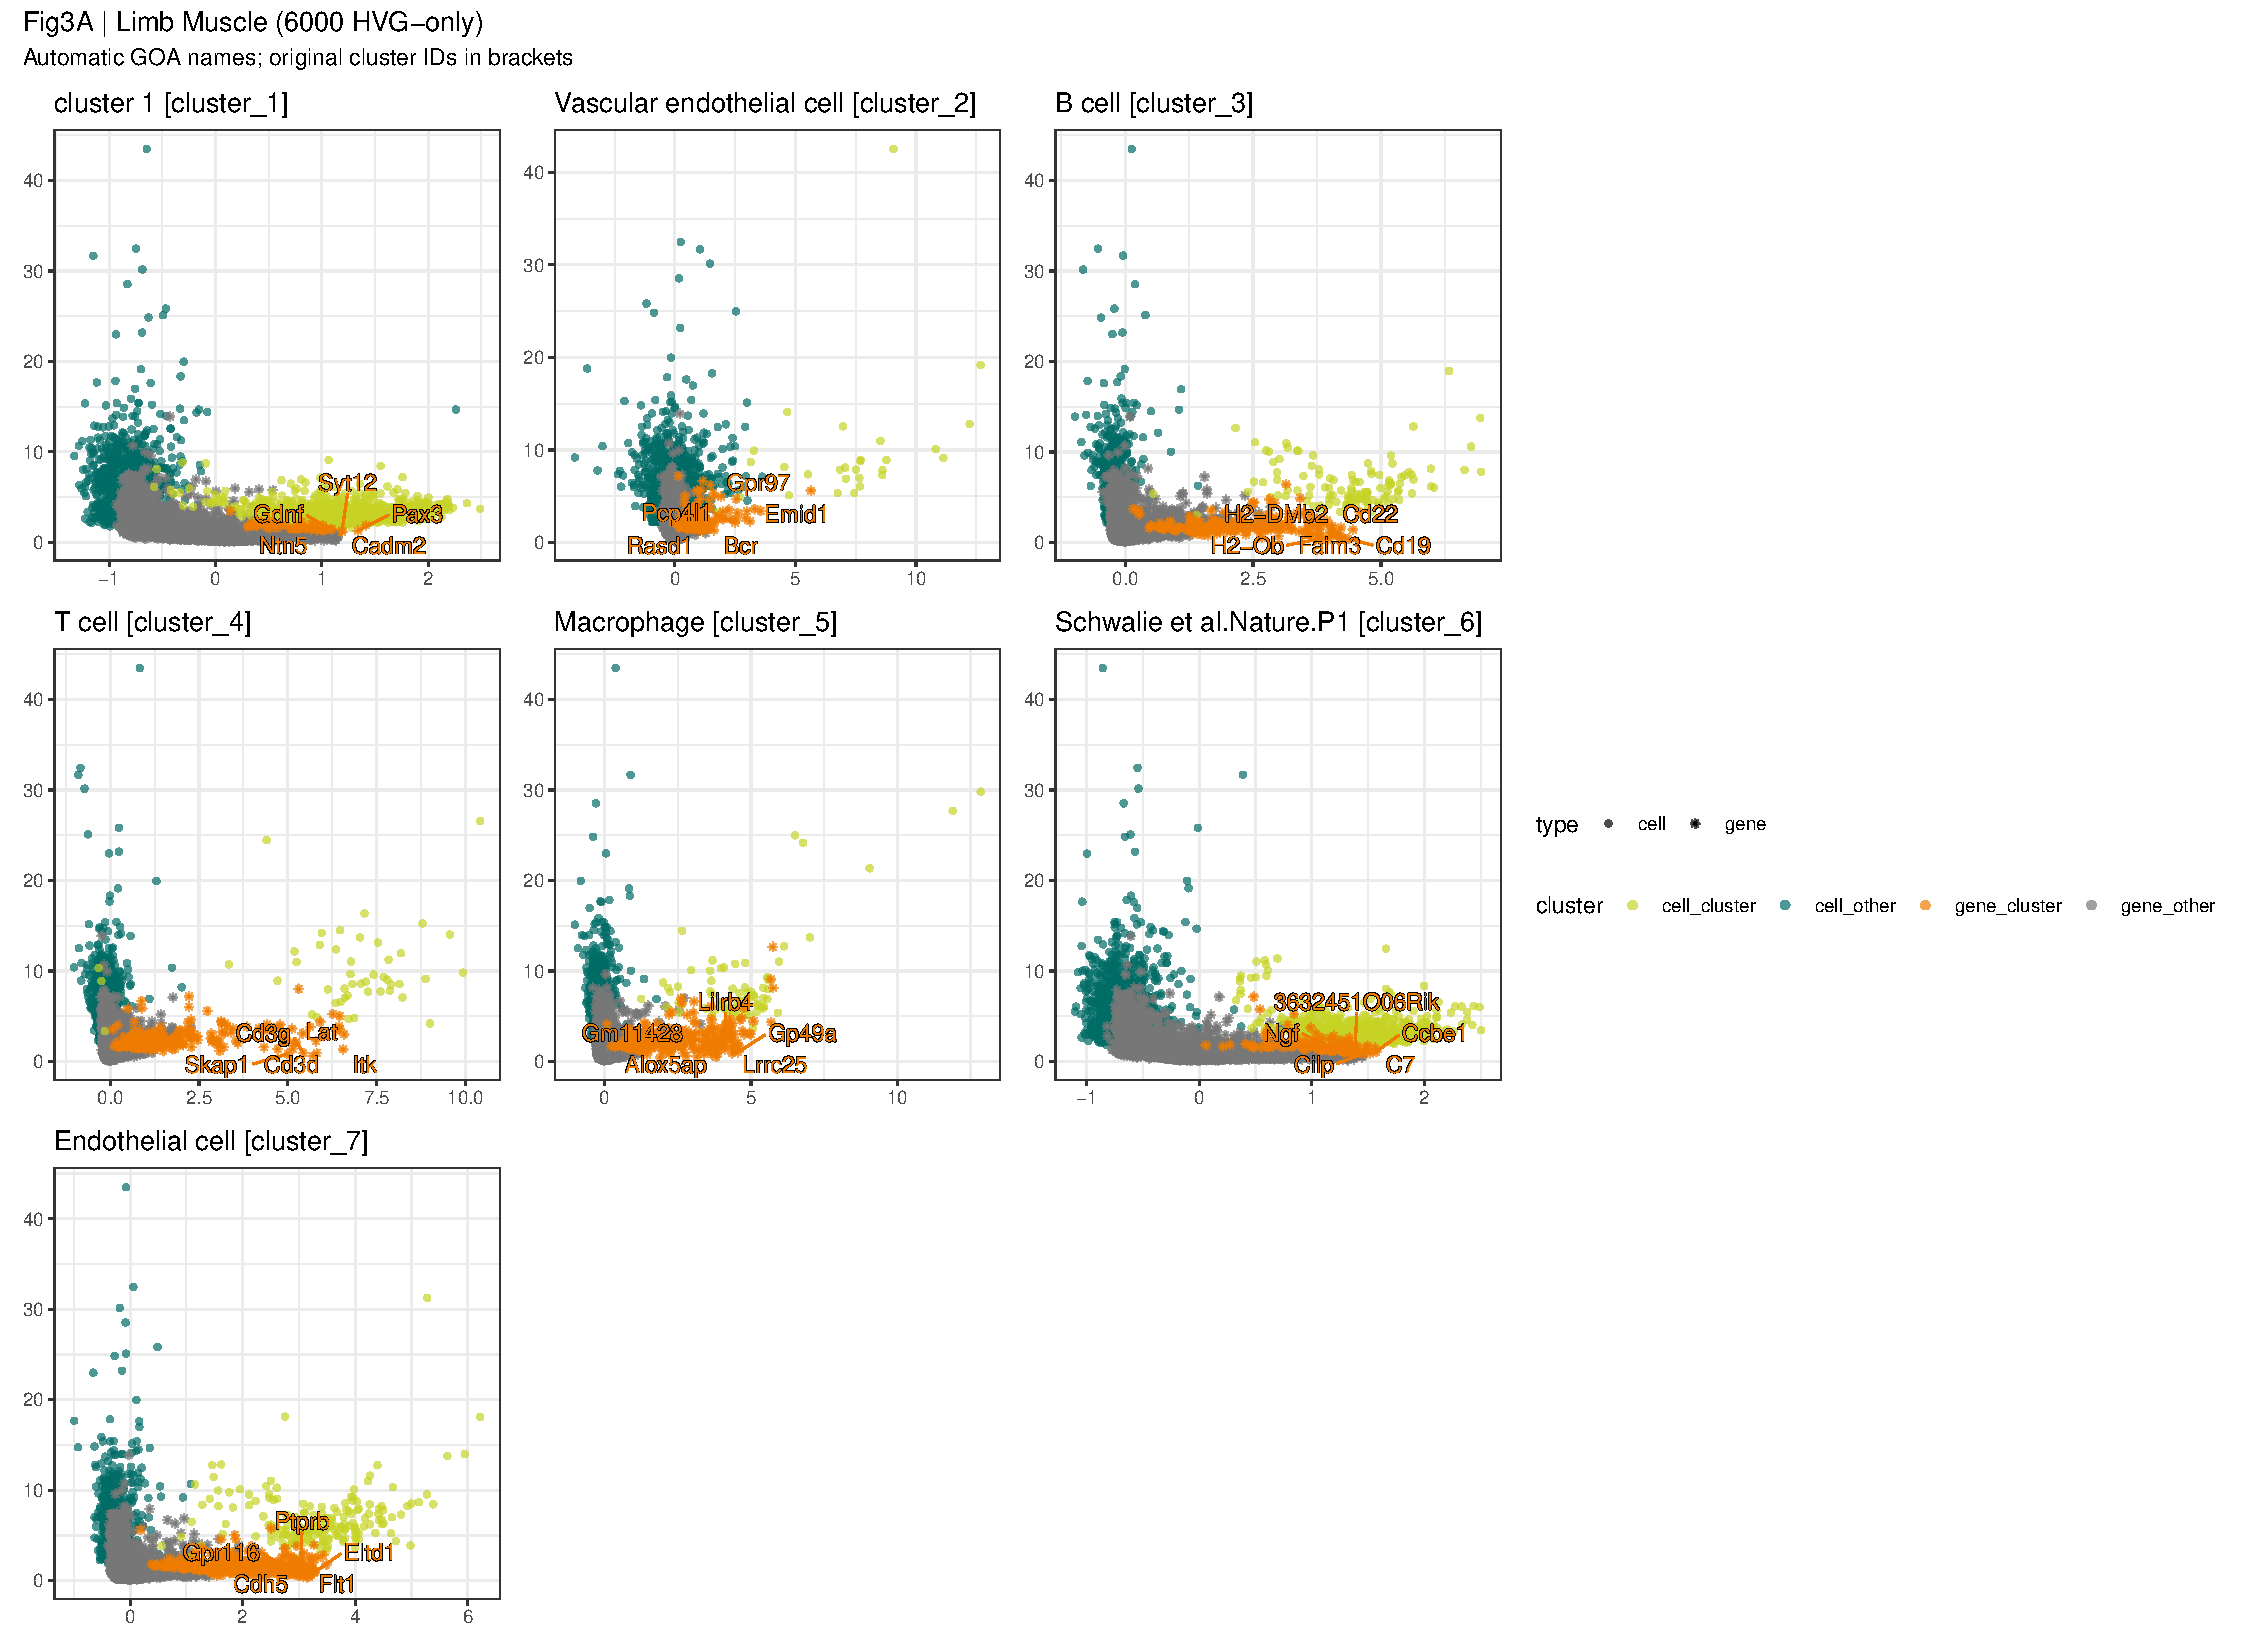
\includegraphics[width=0.96\textwidth,height=0.72\textheight,keepaspectratio]{figures/Fig3A_association_top5.pdf}
\caption{LM七簇关联图与真实top5基因（对应原论文Fig3A）}\label{fig:1}
\end{figure*}

基因得分将投影强度和偏离距离结合。{\ttfamily\nolinkurl{cluster_1}}前五名为Cadm2、Syt12、Ntn5、Pax3、Gdnf，其得分依次为−0.230963、−0.258898、−0.288689、−0.347069、−0.382294。这组负分数说明：在该簇的当前alpha下，正交距离惩罚大于投影收益；图中top5表示簇内排序最高的五个基因。完整分数表支持逐个基因解释。

\subsection{Fig3B/C：免疫与内皮方向}
图~\ref{fig:2}展示B细胞预测簇及T细胞、巨噬细胞方向，图~\ref{fig:3}展示两个内皮预测方向。B与T方向夹角为\allowbreak{}63.9984377°，B与巨噬细胞为\allowbreak{}72.6956194°；两个内皮方向夹角为\allowbreak{}66.1100659°。等比例坐标轴便于观察投影几何。

\begin{figure*}[!tbp]
\centering
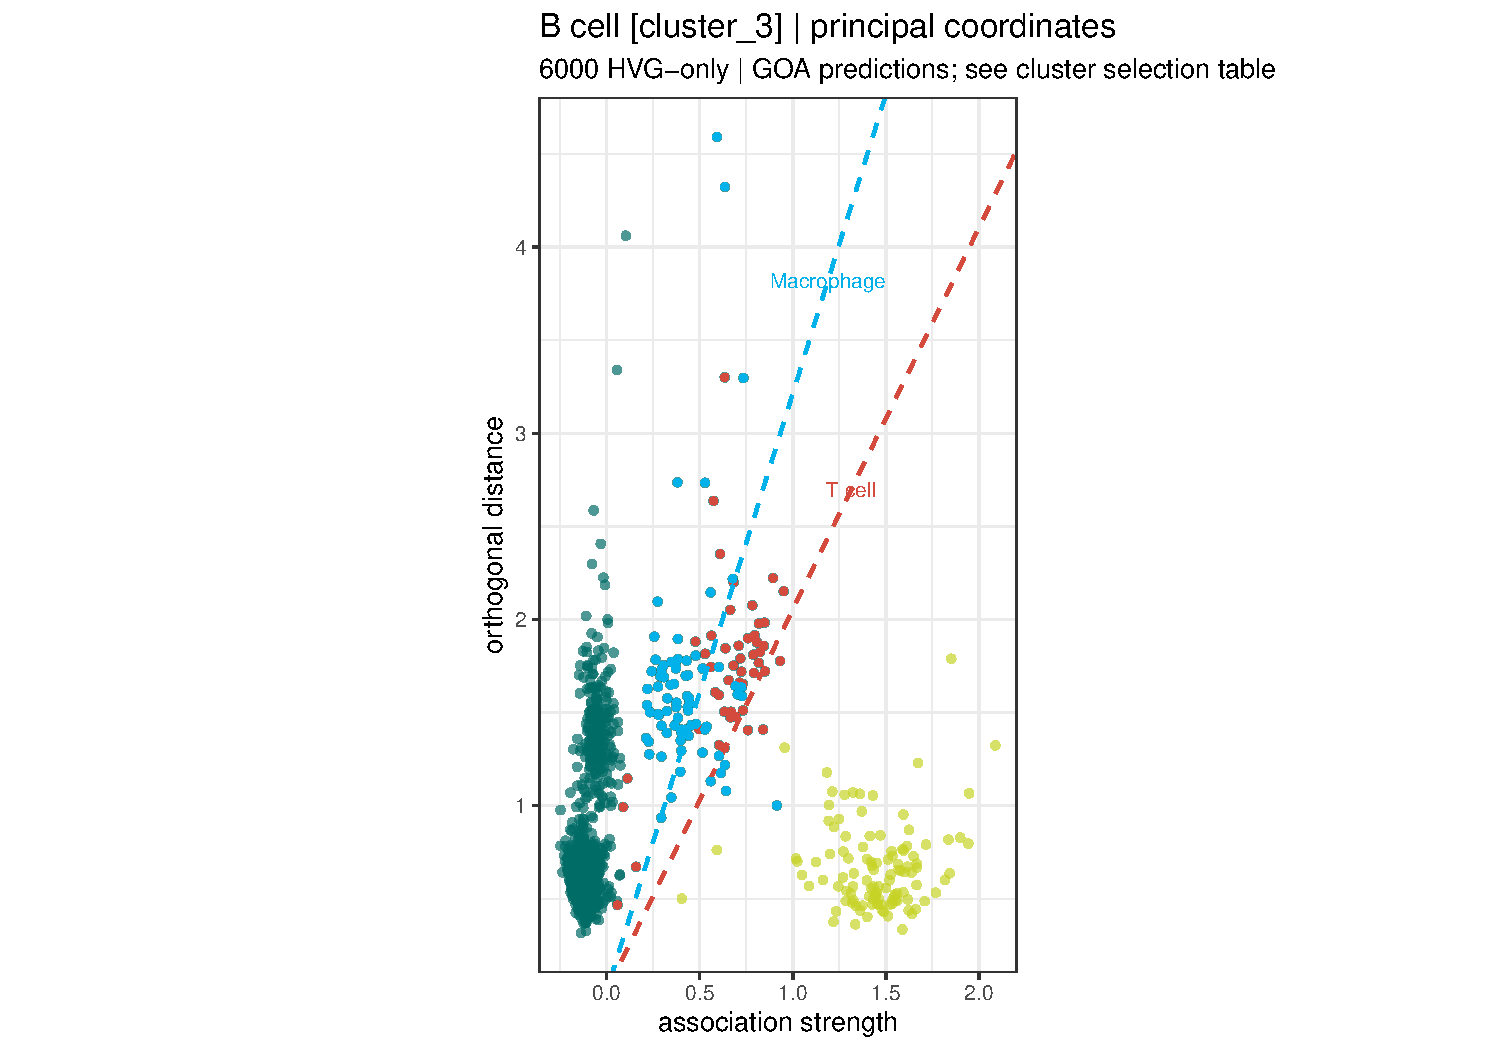
\includegraphics[width=0.96\textwidth,height=0.72\textheight,keepaspectratio]{figures/Fig3B_Bcell_principal.pdf}
\caption{B细胞簇及T细胞、巨噬细胞的主坐标方向比较（对应Fig3B）}\label{fig:2}
\end{figure*}

\begin{figure*}[!tbp]
\centering
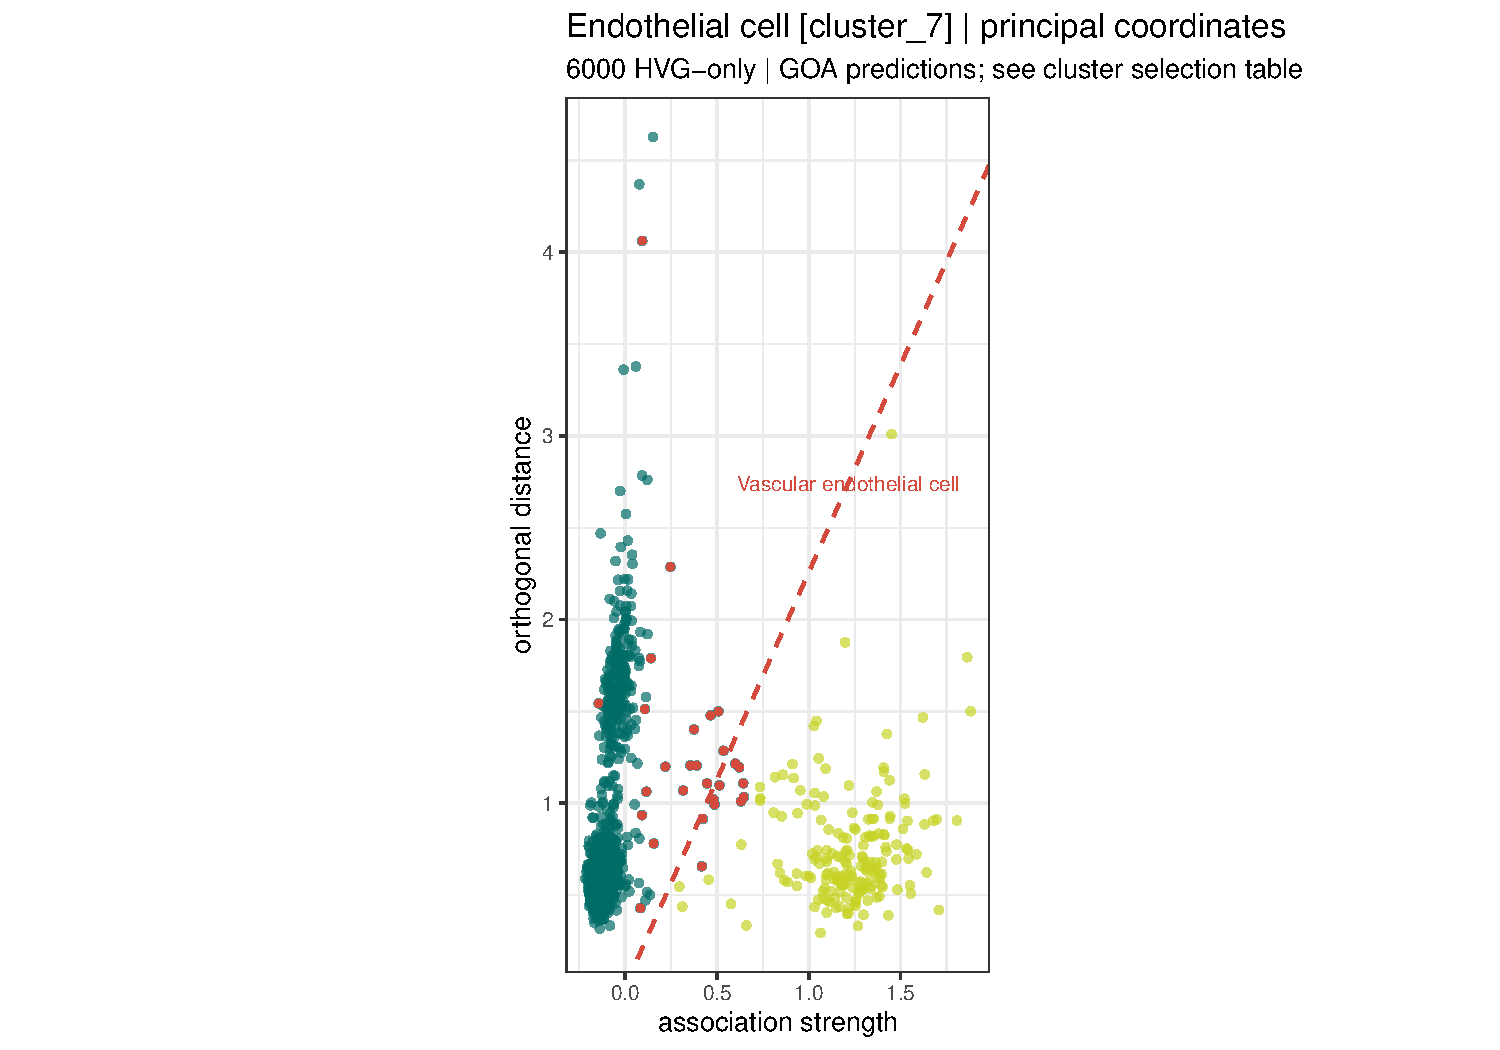
\includegraphics[width=0.96\textwidth,height=0.72\textheight,keepaspectratio]{figures/Fig3C_endothelial_principal.pdf}
\caption{两个内皮预测方向的主坐标比较（对应Fig3C）}\label{fig:3}
\end{figure*}

预测与参考的对应进一步解释了图形。B预测簇含\allowbreak{}113个细胞，其中\allowbreak{}63个原参考为B cell、49个为lymphocyte。Macrophage预测簇\allowbreak{}76个细胞中\allowbreak{}73个参考为macrophage。Endothelial预测簇\allowbreak{}187个细胞均为endothelial cell参考，Vascular endothelial预测簇\allowbreak{}28个细胞中\allowbreak{}19个为该参考。两个内皮方向的细分来自GOA预测；原参考对它们使用同一个endothelial类别。

\subsection{Fig3D：实际拆分合并过程}
图~\ref{fig:4}来自保存的真实成员和方向历史，包含\allowbreak{}22个节点、23条边，21个非根节点均有阶段成员、方向和注释记录。每一层对应有拆分或合并的迭代，各节点内的关联图展示该阶段的细胞分布。

\begin{figure*}[!tbp]
\centering
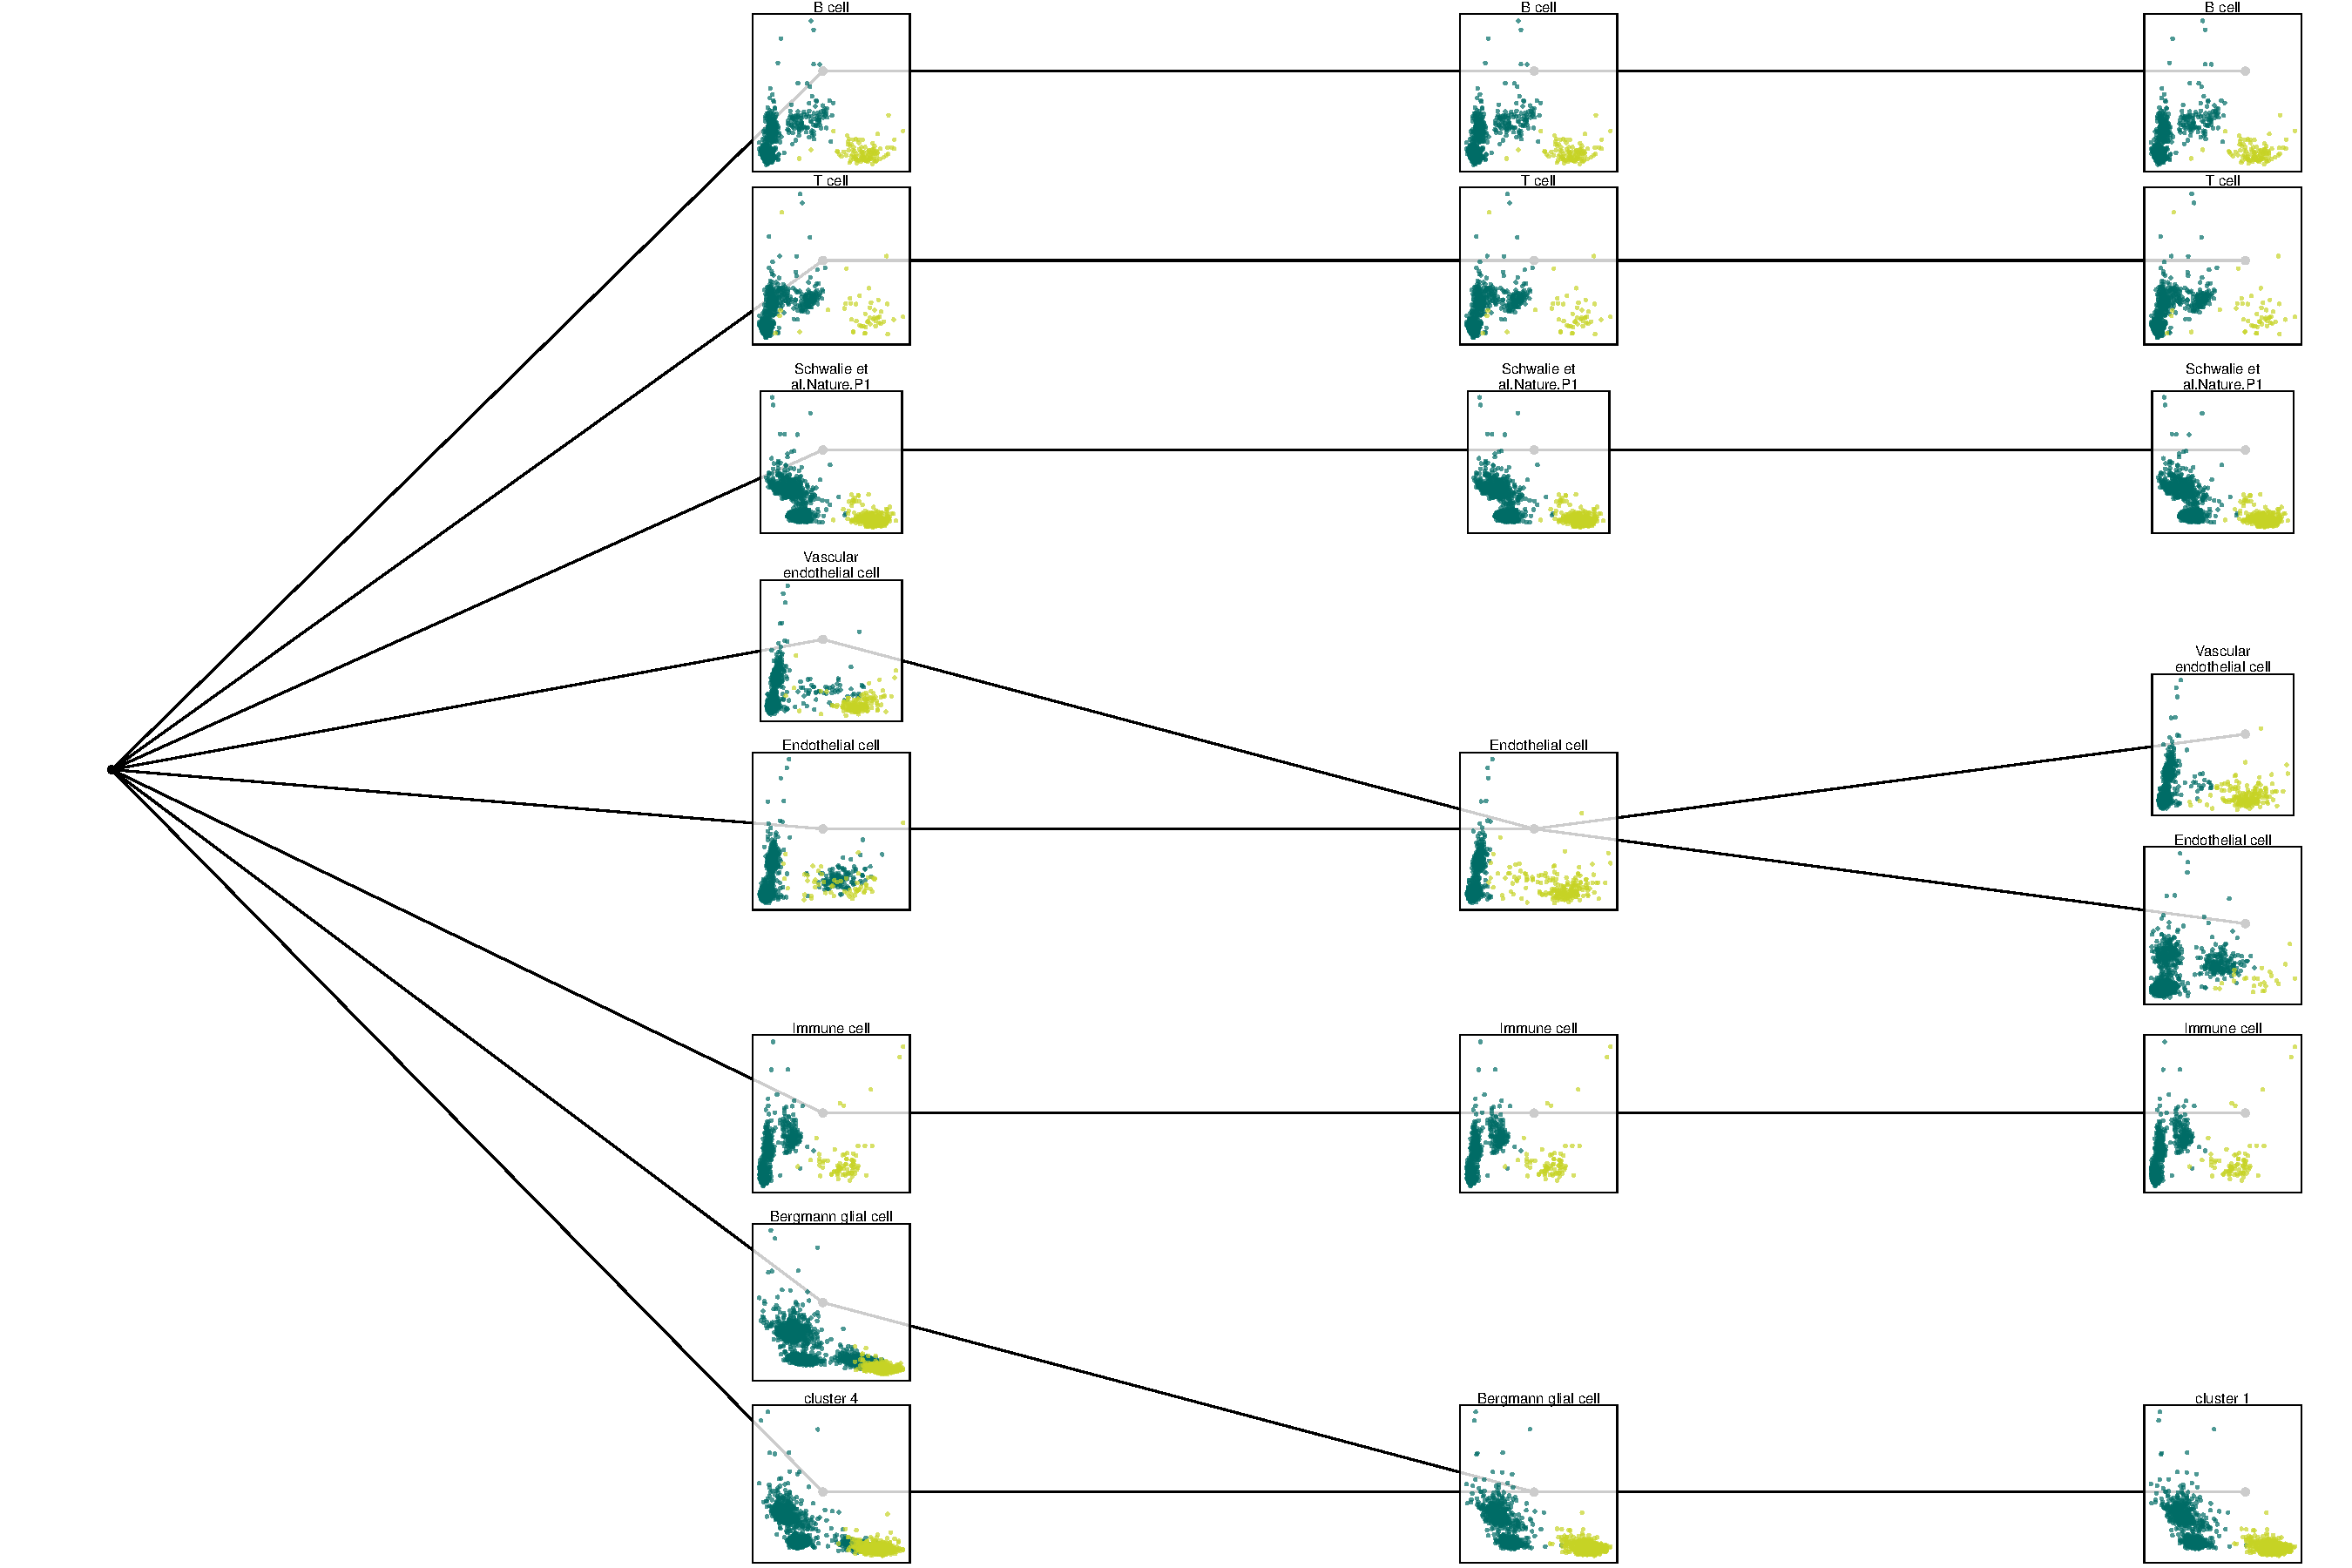
\includegraphics[width=0.96\textwidth,height=0.72\textheight,keepaspectratio]{figures/Fig3D_actual_split_merge_history.pdf}
\caption{LM真实拆分合并历史（对应Fig3D）}\label{fig:4}
\end{figure*}

历史图使用{\ttfamily\nolinkurl{keep_end=FALSE}}展示到最后一次拆分，最终成员表则来自随后的细化。因此一个末层\allowbreak{}25细胞分支与最终\allowbreak{}28细胞簇分别代表不同计算时点。历史注释保留Immune cell、Bergmann glial cell等上游预测名称，反映当时的基因富集结果。该图把初始\allowbreak{}8方向到最终\allowbreak{}7簇的调整过程与细胞几何联系起来。

\subsection{S1A/B：全部方向的定量关系}
图~\ref{fig:5}给出\allowbreak{}7×7两两方向角矩阵，图~\ref{fig:6}将七个基准关联图及其他方向投影组织成\allowbreak{}49个面板。前者适合读出明确角度，后者便于比较同一基准下其他簇的投影位置。

\begin{figure*}[!tbp]
\centering
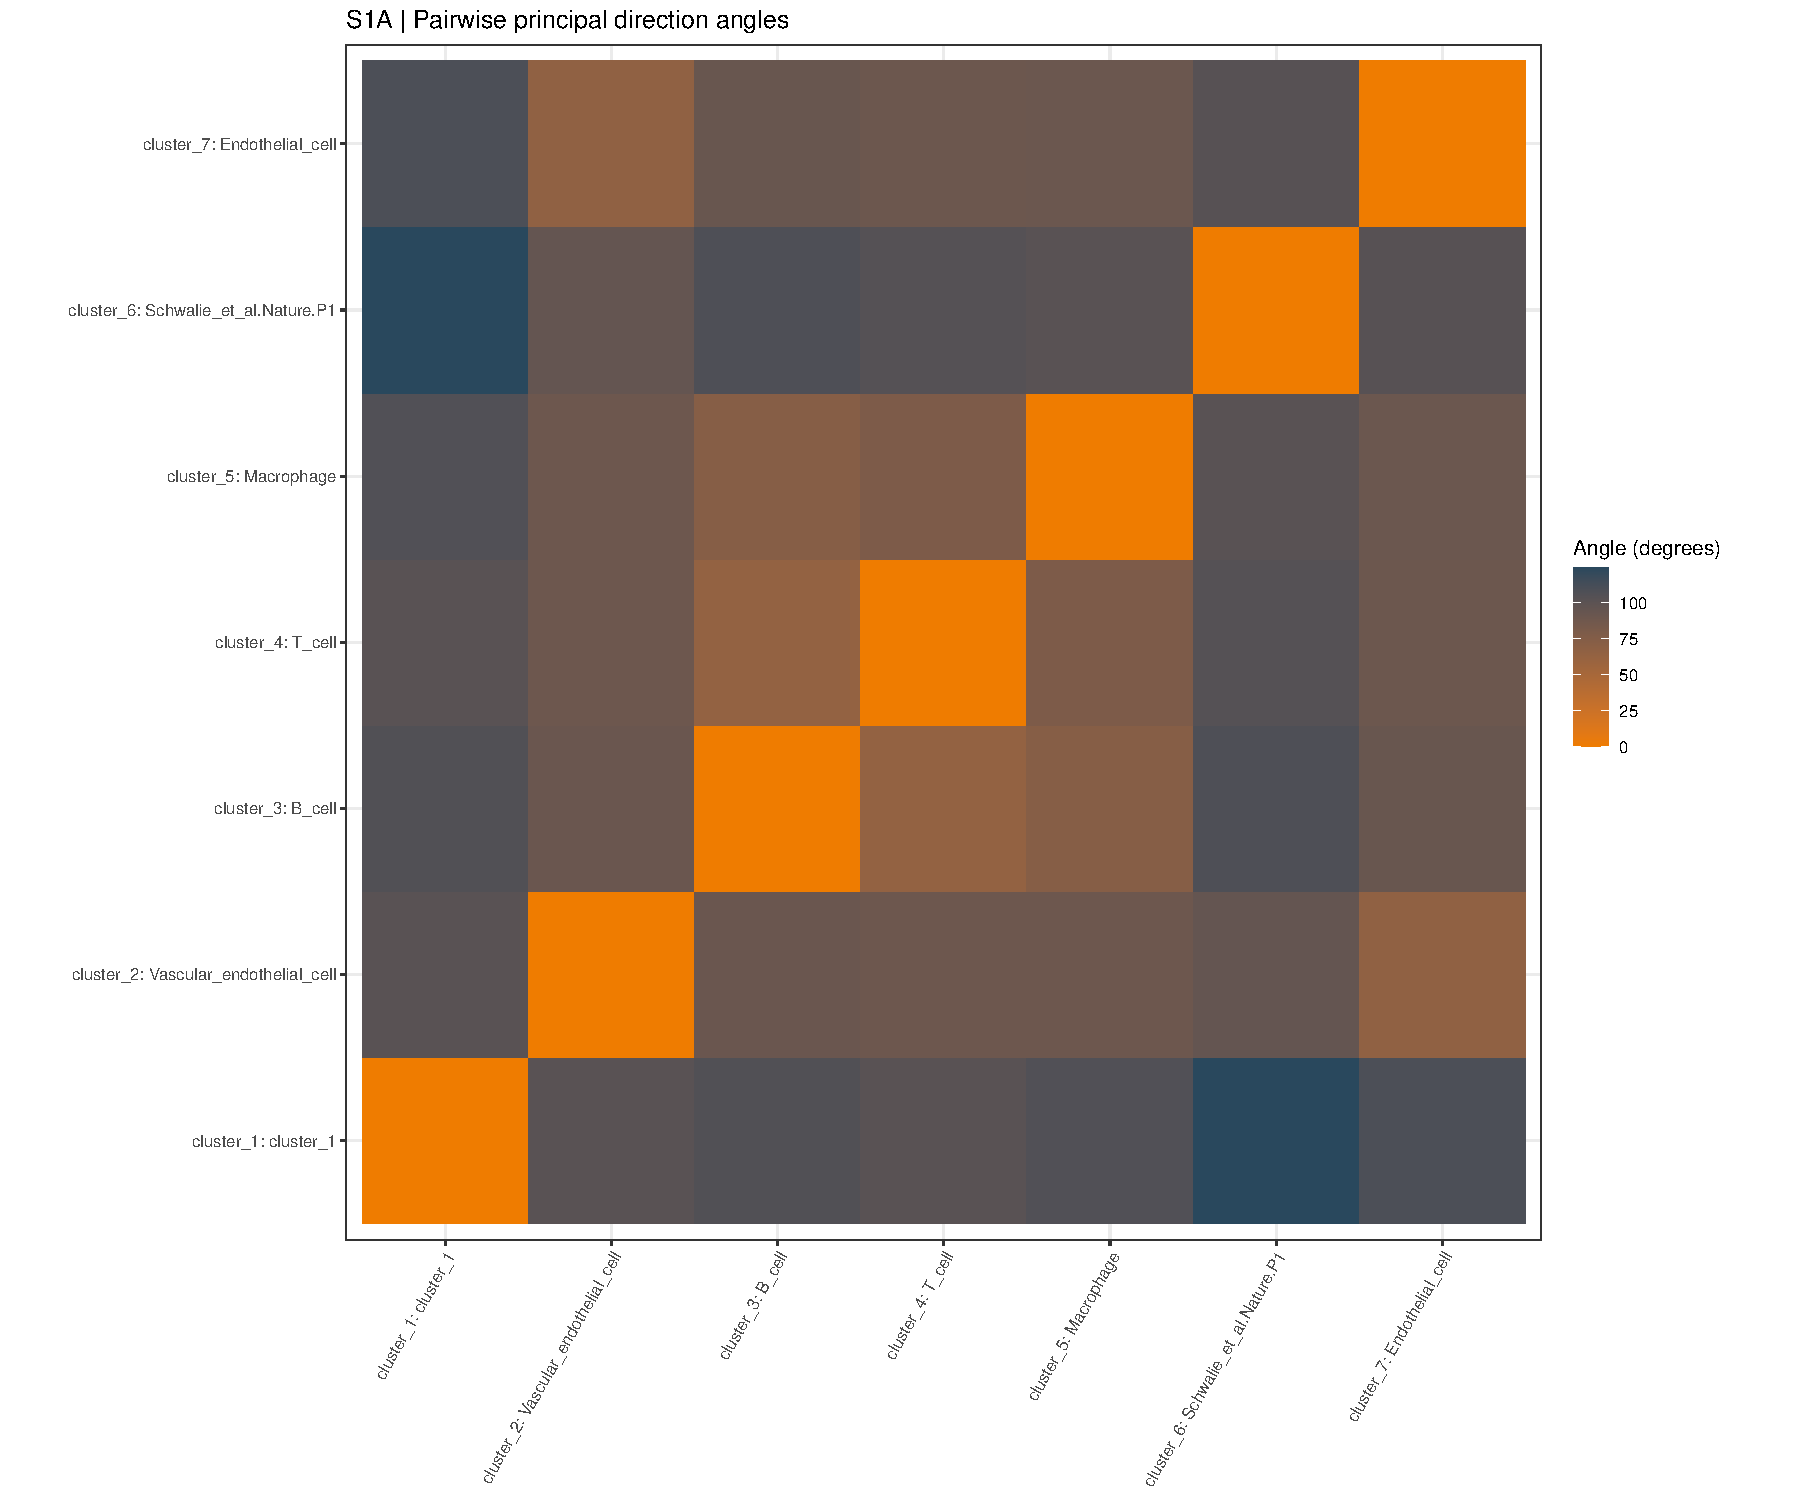
\includegraphics[width=0.96\textwidth,height=0.72\textheight,keepaspectratio]{figures/S1A_direction_angle_heatmap.pdf}
\caption{全部簇方向的两两夹角，单位为度（对应S1A）}\label{fig:5}
\end{figure*}

\begin{figure*}[!tbp]
\centering
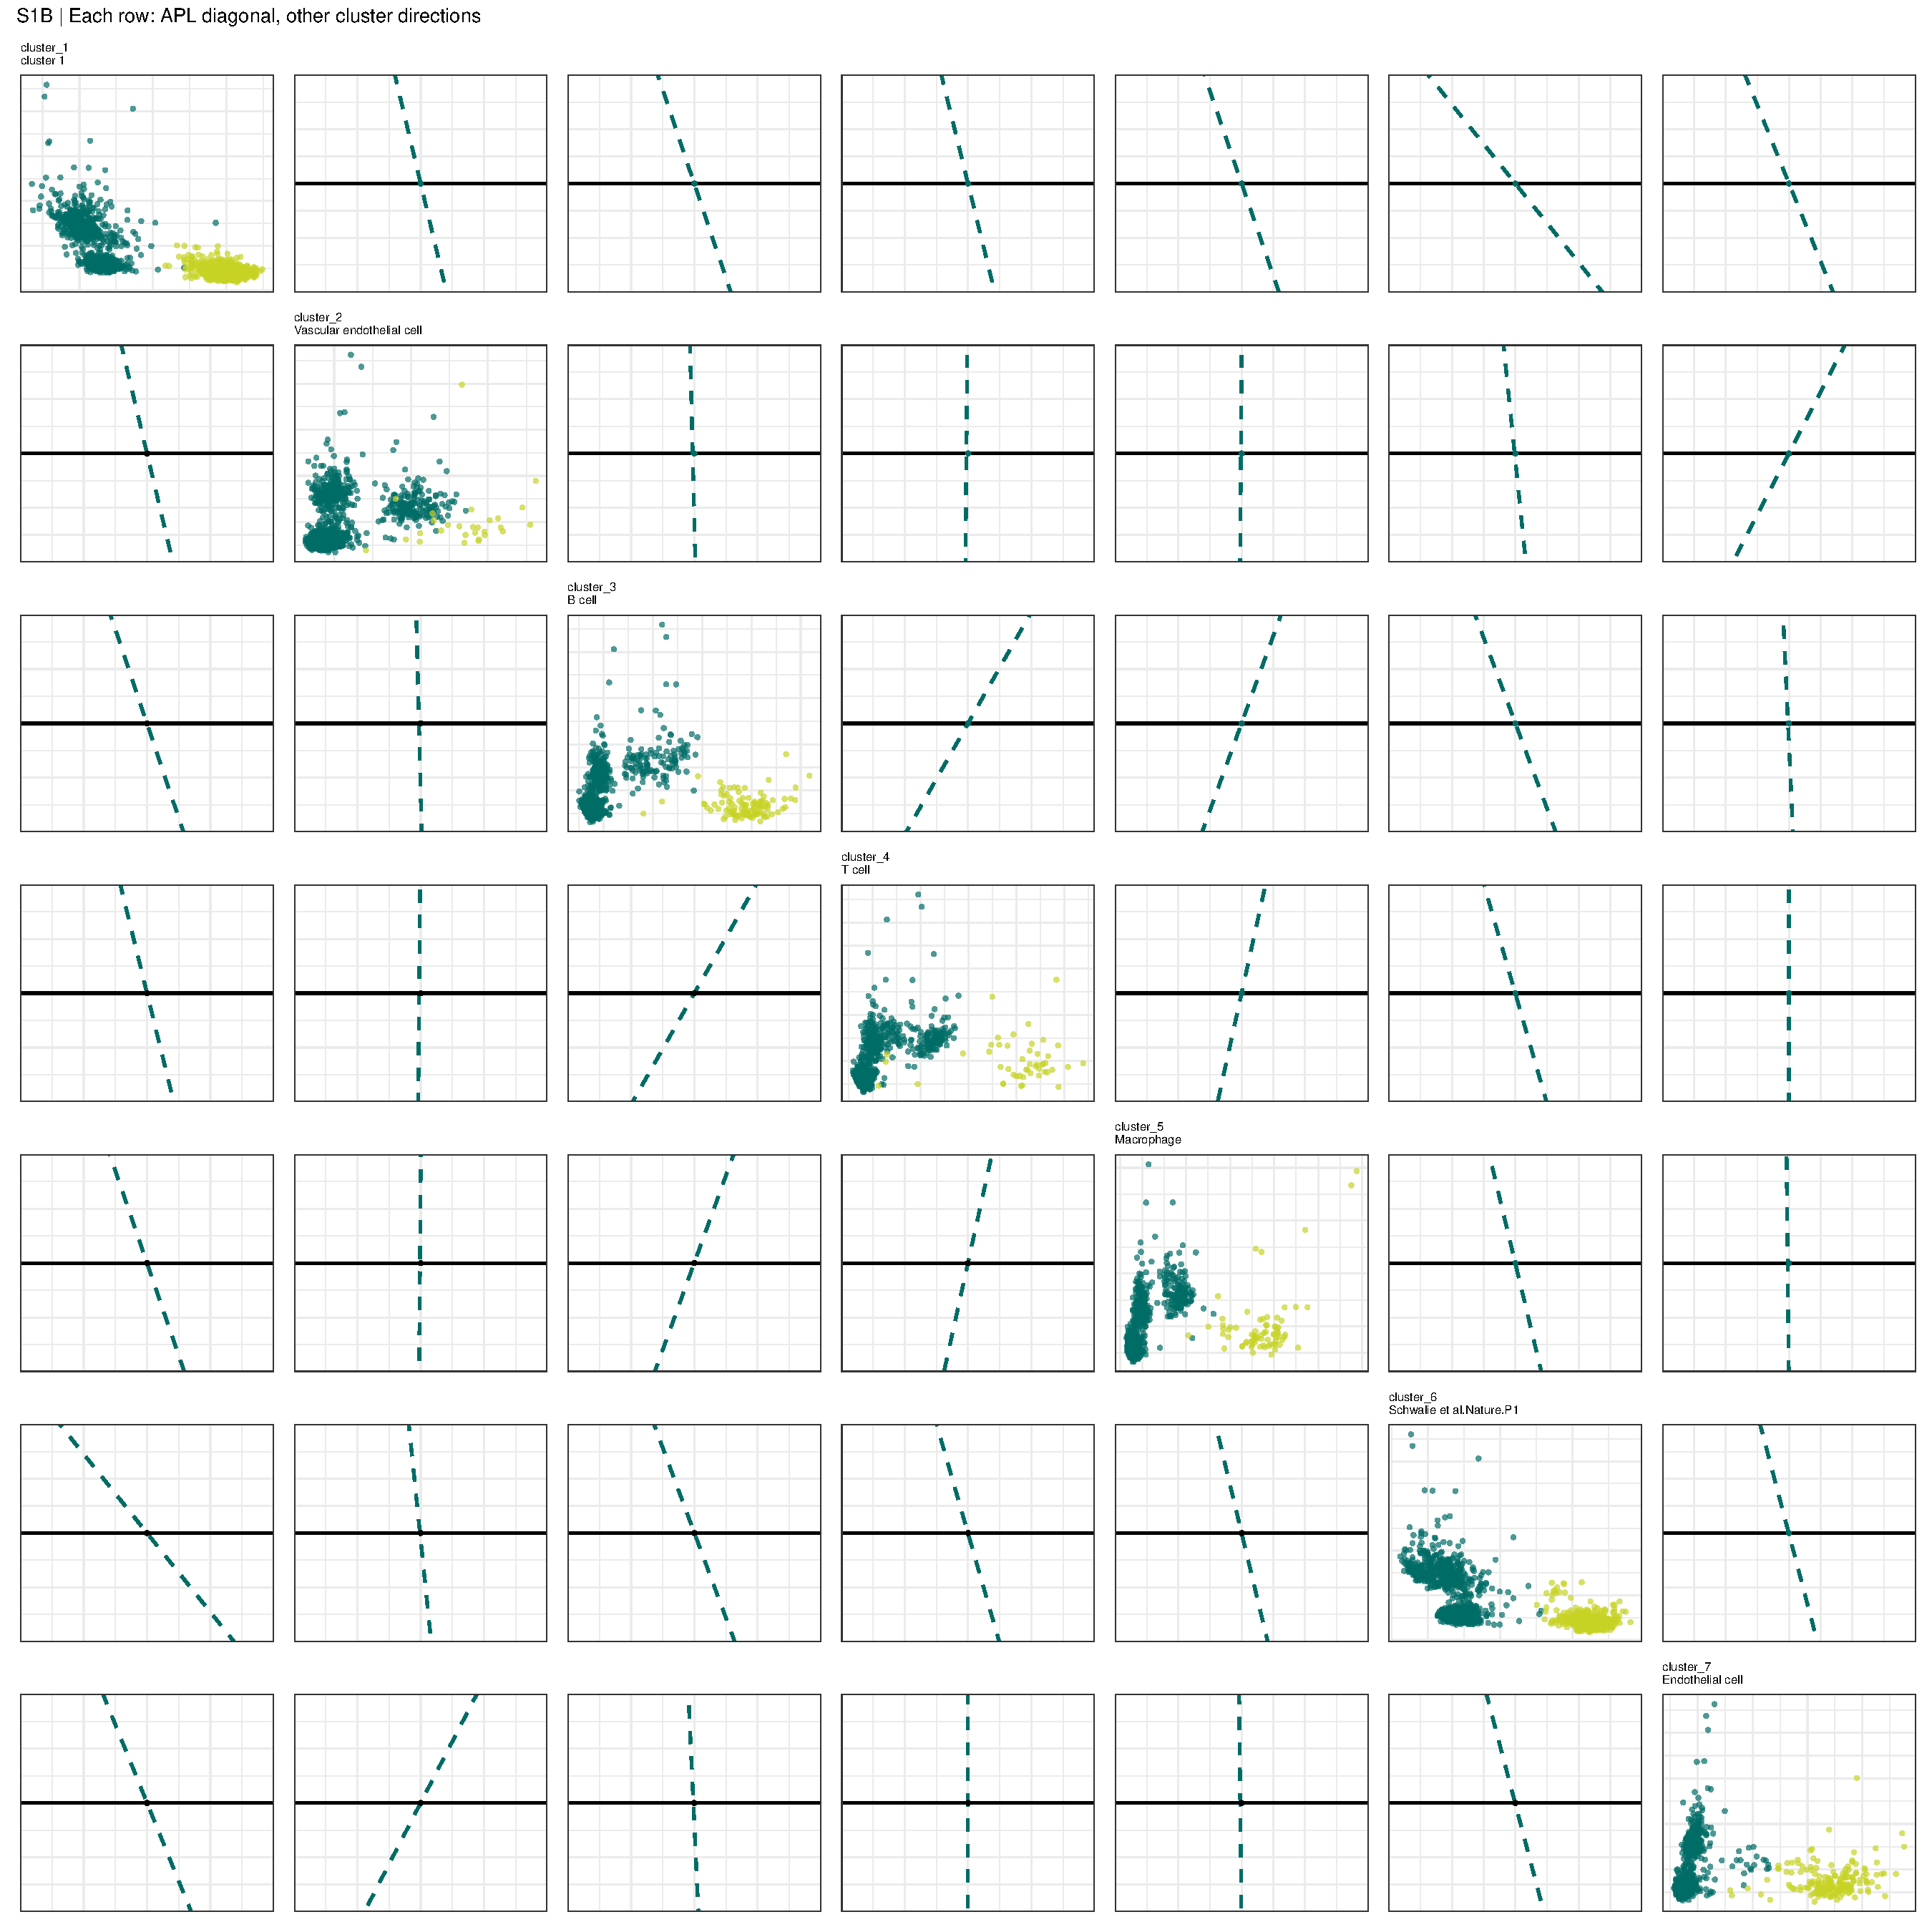
\includegraphics[width=0.96\textwidth,height=0.72\textheight,keepaspectratio]{figures/S1B_direction_projection_matrix.pdf}
\caption{七个基准方向的关联图与方向投影矩阵（对应S1B）}\label{fig:6}
\end{figure*}

方向接近表示表达关联几何相近；结合原参考、自动注释和基因排名，可讨论哪些簇具有相似表达成分。方向角表保存了完整精度，补充了图中面板缩放后的视觉信息。

\subsection{S1C：预测分区与参考标签}
图~\ref{fig:7}保留\allowbreak{}1882个细胞在七个预测簇与八类原参考之间的全部流量。流量表、列联表和指标使用相同细胞ID，因此可以从总体ARI进一步定位到具体类别。

\begin{figure*}[!tbp]
\centering
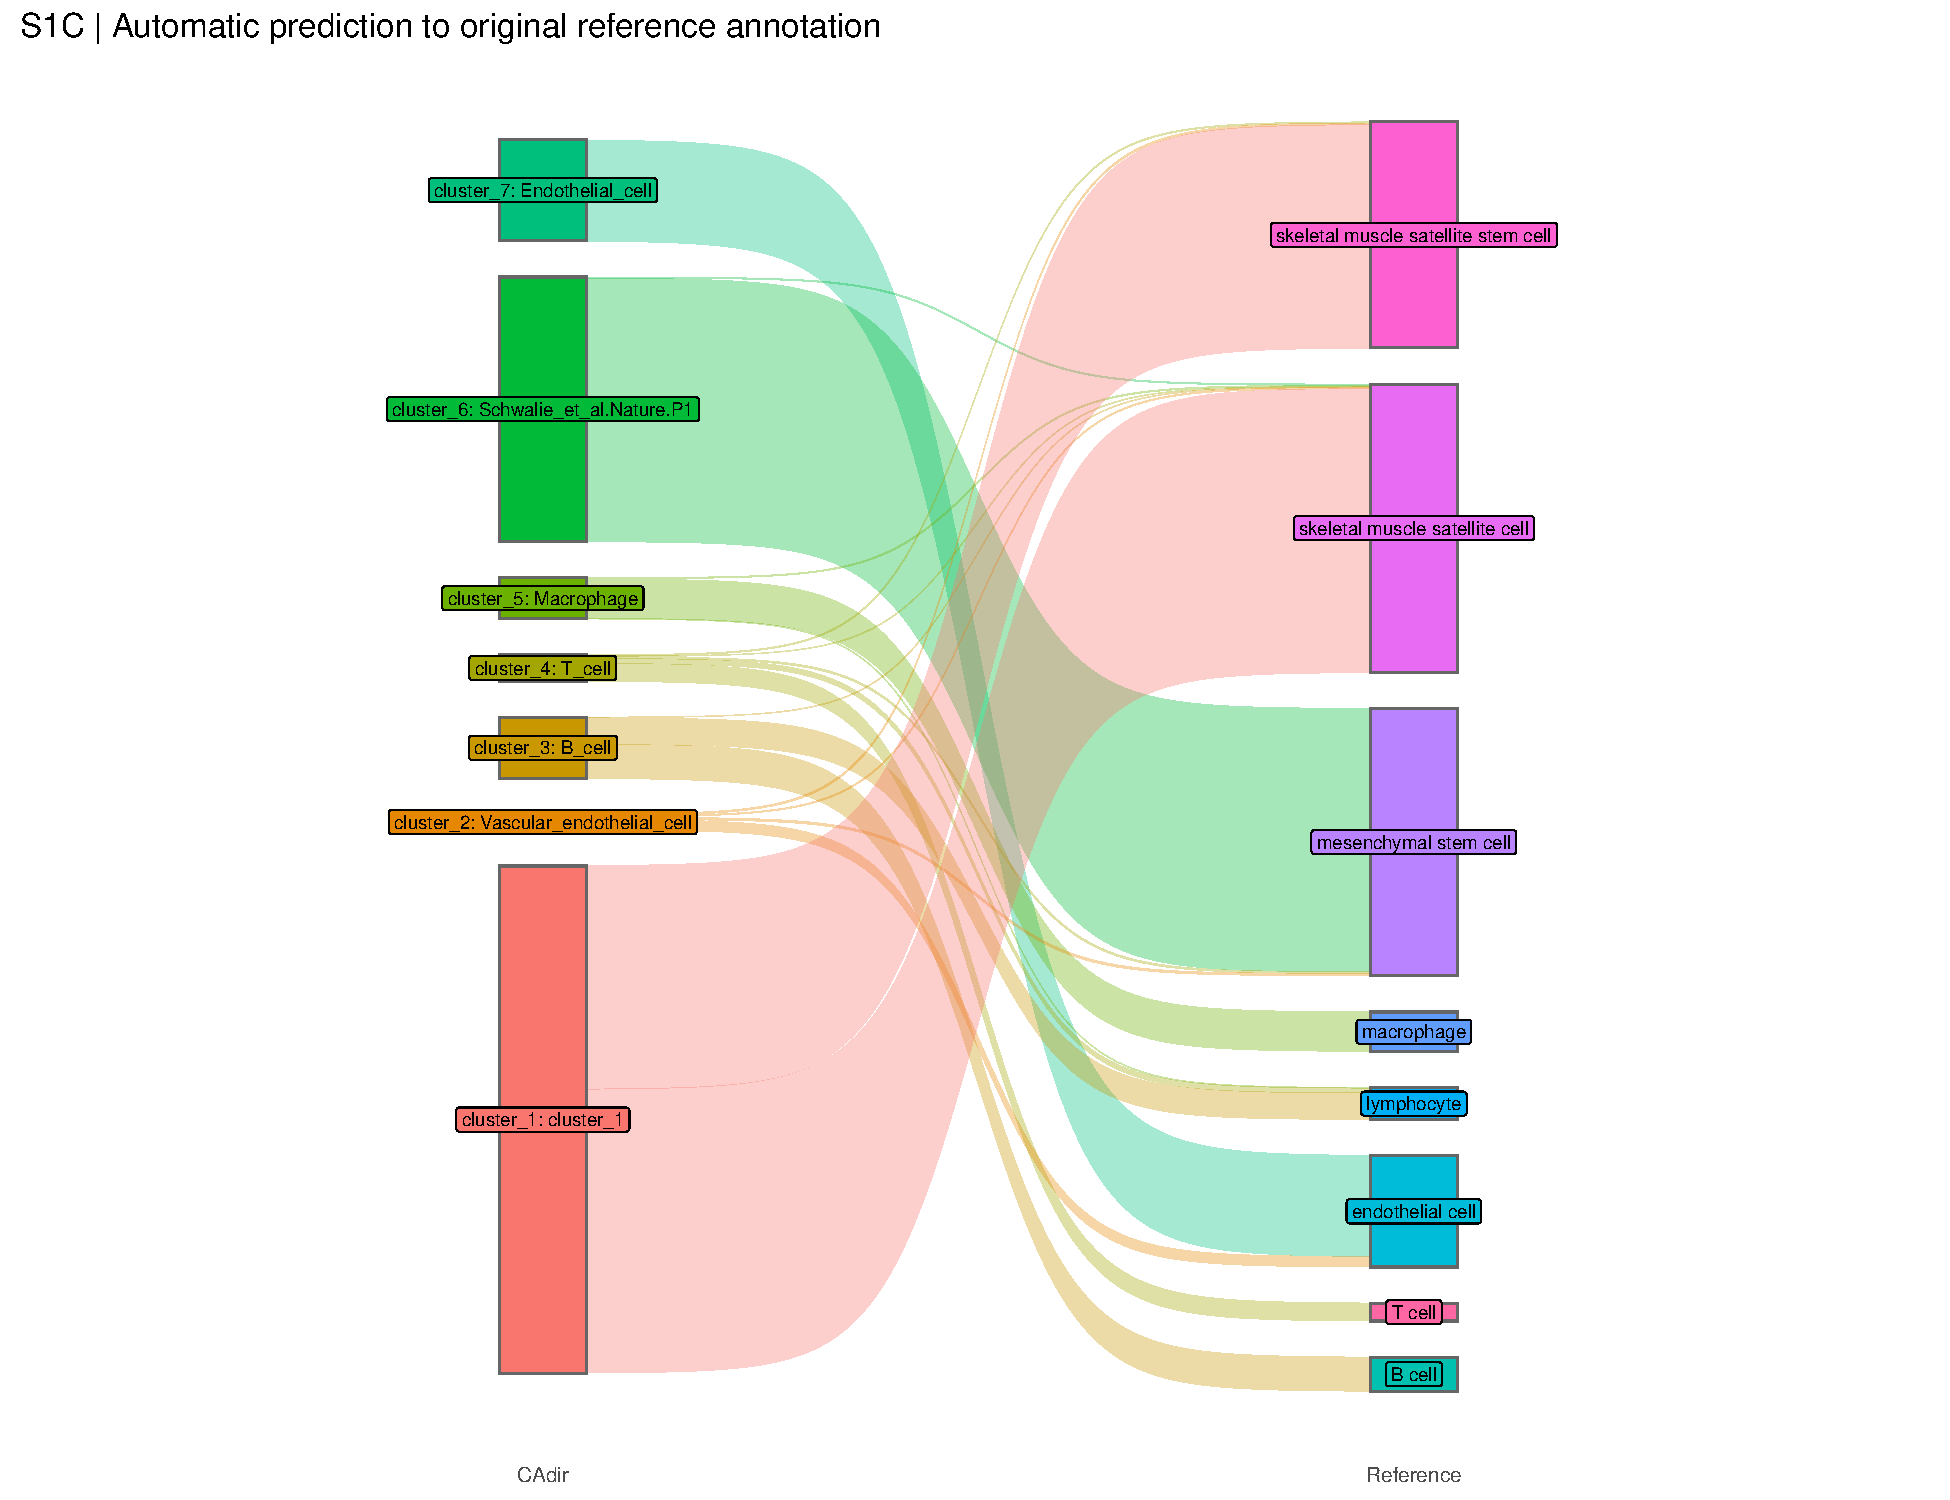
\includegraphics[width=0.96\textwidth,height=0.72\textheight,keepaspectratio]{figures/S1C_reference_sankey.pdf}
\caption{LM七簇与八类原参考的细胞流量（对应S1C）}\label{fig:7}
\end{figure*}

参考重叠显示，{\ttfamily\nolinkurl{cluster_1}}以skeletal muscle satellite cell为最大类别（526／940），Schwalie命名簇以mesenchymal stem cell为最大类别（488／490）。各簇的组成有不同纯度，解释了总体指标与局部结构之间的关系。自动预测提供基因集层面的注释，参考流量提供已发布标签层面的对应。

\subsection{S1D/E：标准坐标与主坐标}
图~\ref{fig:8}和图~\ref{fig:9}将对应的免疫、内皮展示转换为标准坐标，并叠加相同簇的方向。方向按奇异值逐轴转换，细胞与方向坐标由实际对象计算。

\begin{figure*}[!tbp]
\centering
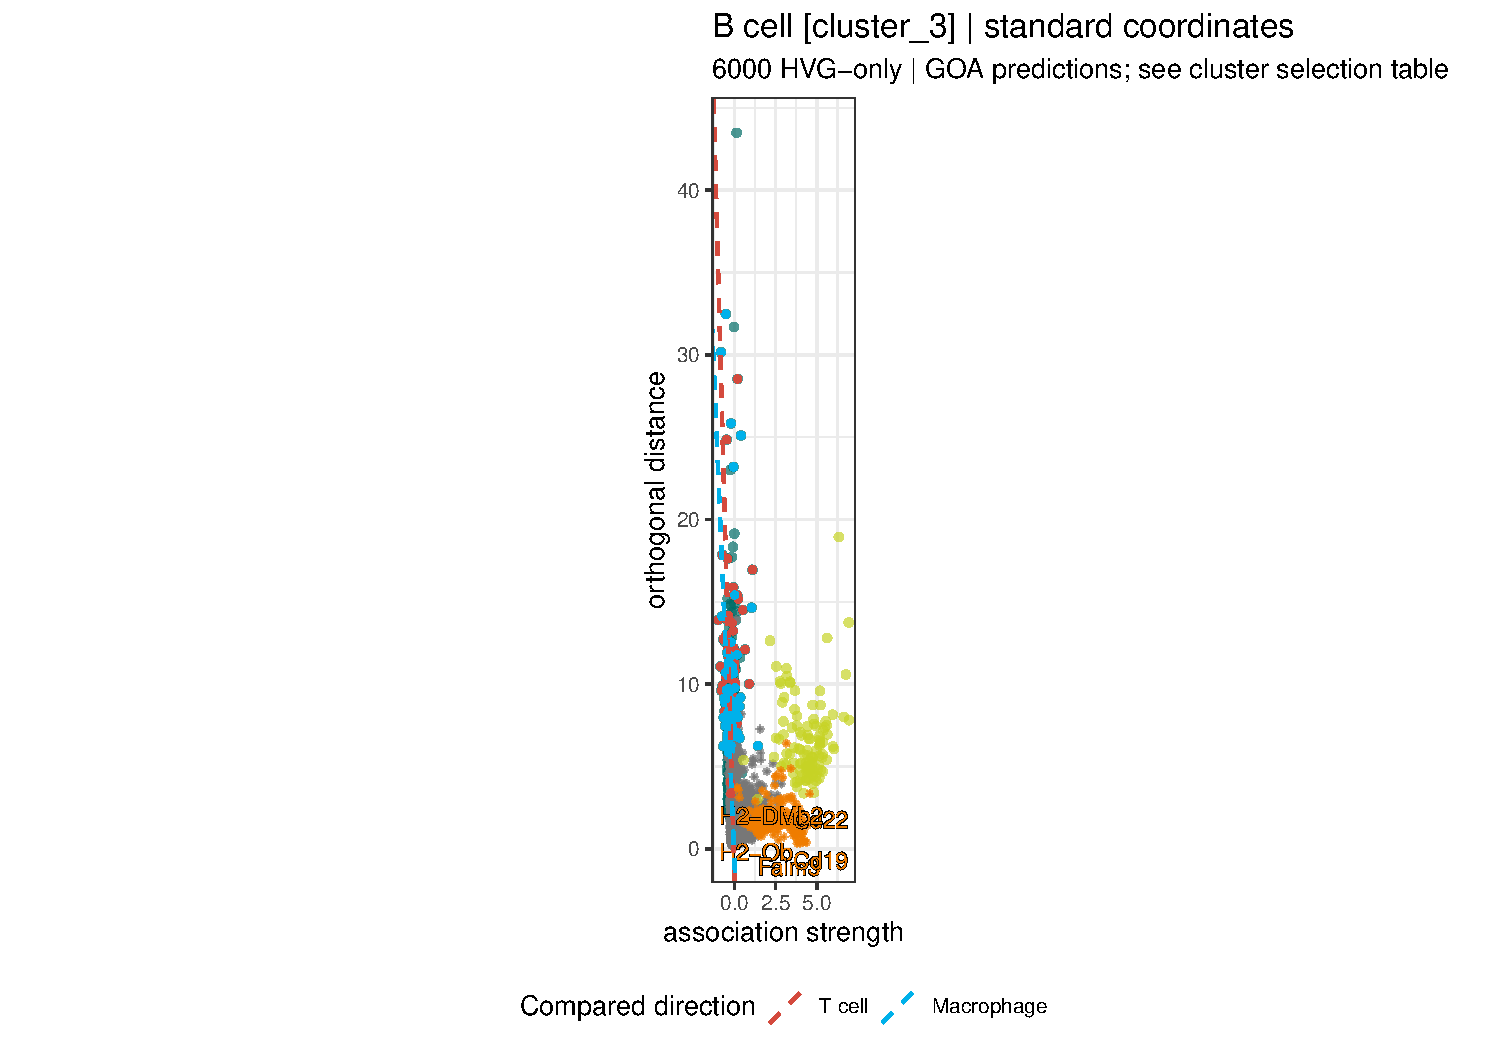
\includegraphics[width=0.96\textwidth,height=0.72\textheight,keepaspectratio]{figures/S1D_Bcell_standard.pdf}
\caption{免疫方向的标准坐标关联图（对应S1D）}\label{fig:8}
\end{figure*}

\begin{figure*}[!tbp]
\centering
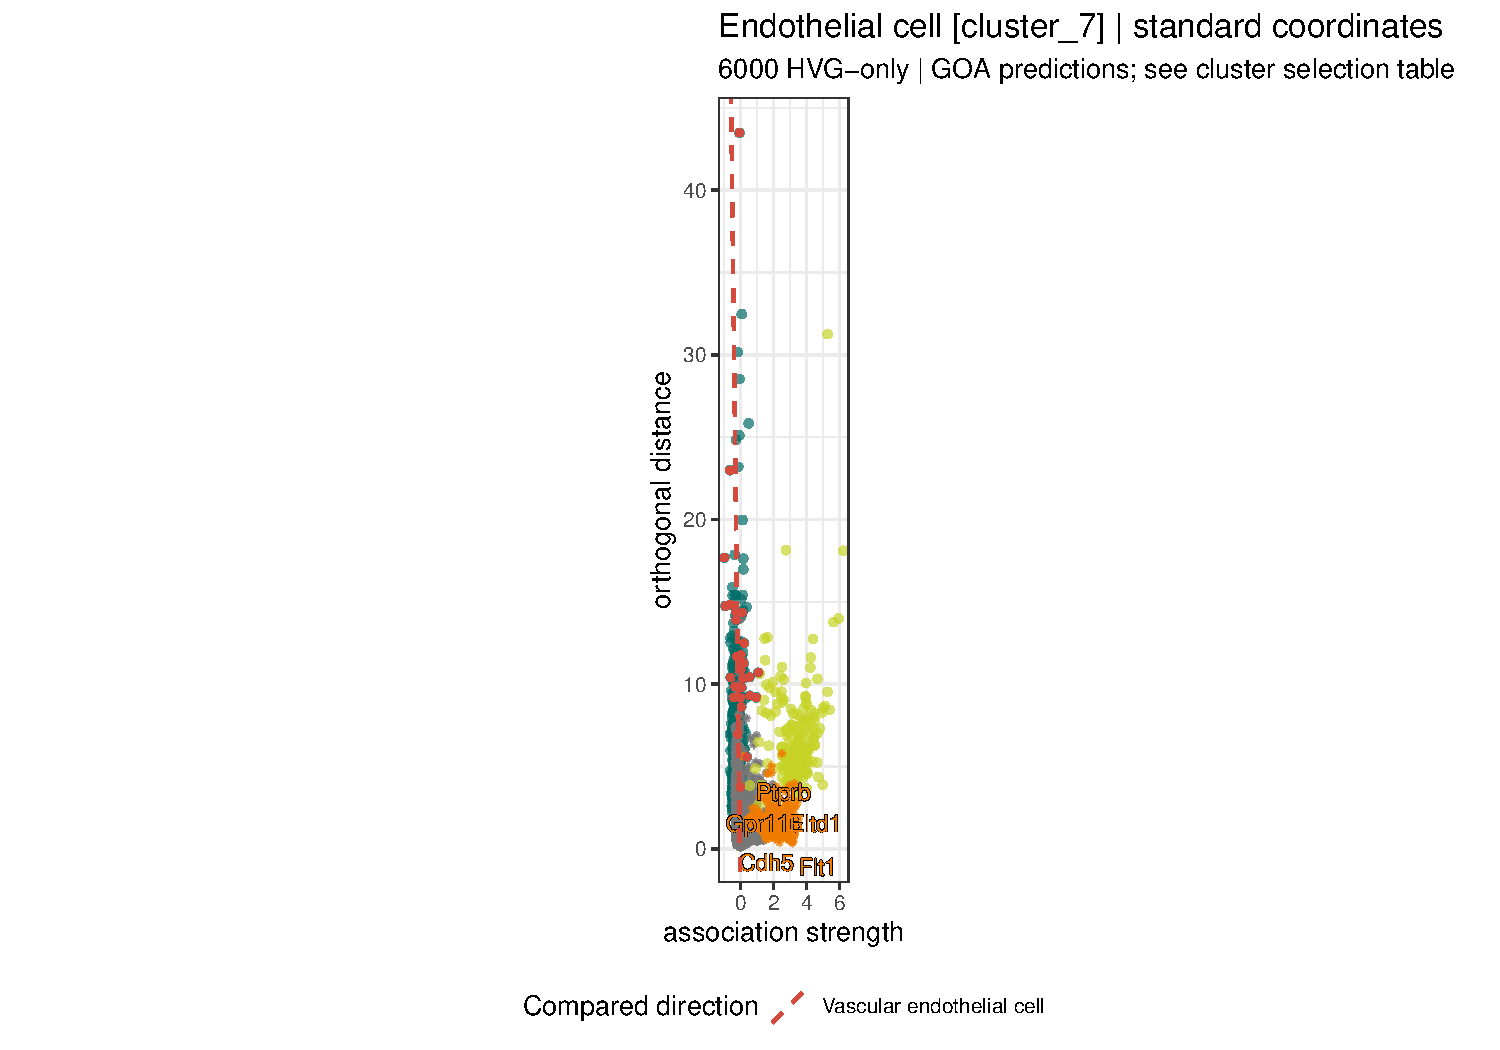
\includegraphics[width=0.96\textwidth,height=0.72\textheight,keepaspectratio]{figures/S1E_endothelial_standard.pdf}
\caption{内皮方向的标准坐标关联图（对应S1E）}\label{fig:9}
\end{figure*}

两组比较中的最大角度变化为\allowbreak{}27.5359338°。这一结果展示了各轴缩放如何改变方向关系。主坐标图用于解释原聚类方向角，标准坐标图用于观察与联合显示基因相联系的坐标表达。修复后的底部图例完整显示比较方向。

\subsection{资源记录与数值检查}
LM本次真实案例进程耗时\allowbreak{}36.3743秒，R进程峰值RSS为\allowbreak{}2278652 KiB，约\allowbreak{}2.173 GiB。阶段记录中，CA为\allowbreak{}6.535秒，CAdir为\allowbreak{}3.770秒；进程总耗时还包括读取、检查、排名、注释及导出。

独立检查从保存对象重算CA与关联图坐标、1200个基因分数及排名、ARI／NMI、GOA超几何与校正概率、Hungarian目标以及历史拓扑。最终图例修复经复验，九图和科学表采用固定提交。通过这些记录，数值、图形和运行对象形成可追溯对应。

\section{HSC新数据对照结果}
\subsection{共同队列与比较设计}
共同QC由\allowbreak{}1920个候选细胞保留\allowbreak{}1656个，得到\allowbreak{}40721个合格基因和\allowbreak{}6000个共享高变基因。两种方法使用相同表达矩阵及\allowbreak{}1641细胞评价集合，各运行五个种子。图~\ref{fig:10}展示质量控制与最终队列组成。

\begin{figure*}[!tbp]
\centering
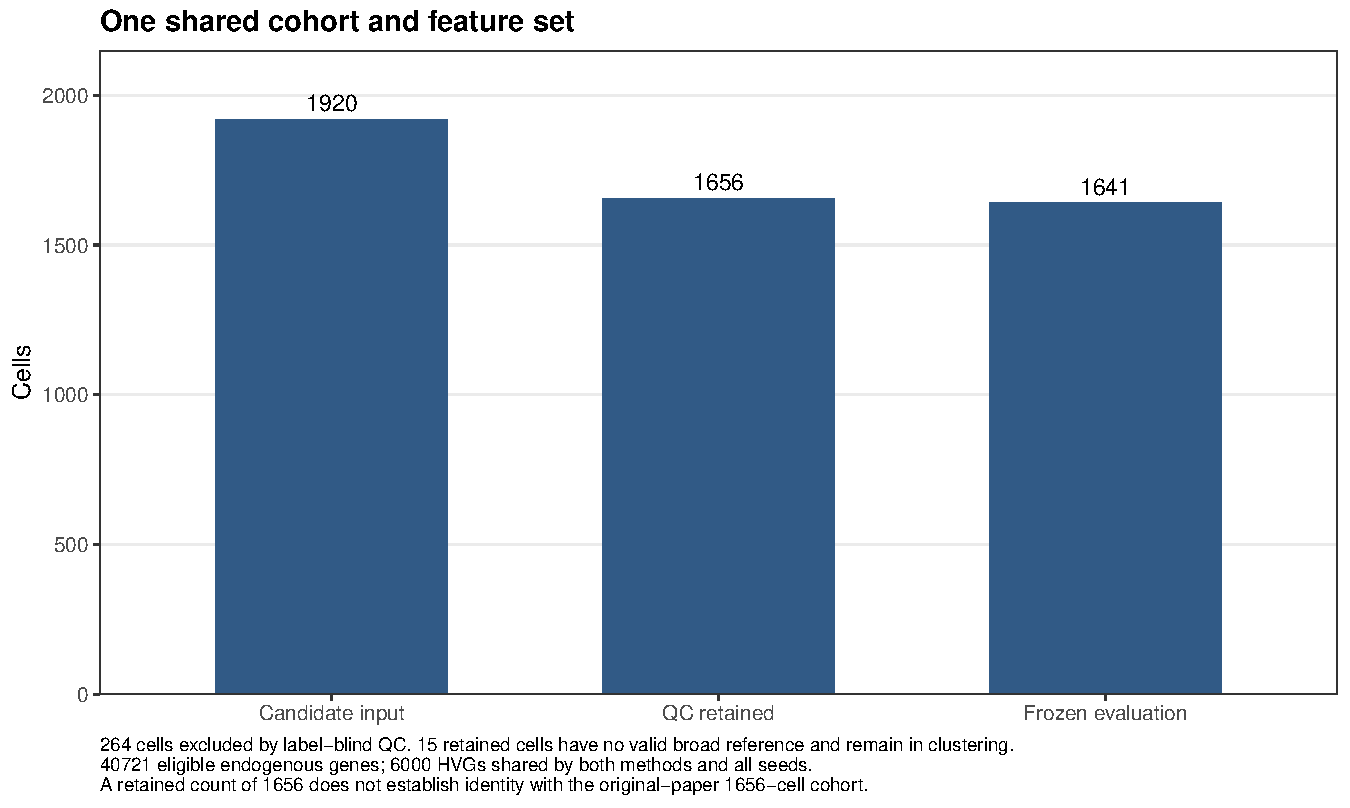
\includegraphics[width=0.96\textwidth,height=0.72\textheight,keepaspectratio]{figures/HSC_04-common-cohort.pdf}
\caption{HSC共同QC与聚类／评价队列组成}\label{fig:10}
\end{figure*}

比较保持了输入、特征、降维维数、参考集合及预定种子的一致；CAdir的方向更新、拆分合并与PCA-SNN-Louvain的社区划分分别按各自配置执行。

\subsection{全部种子的指标}
\begin{table*}[!htbp]
\centering\zihao{-5}
\caption{HSC两方法五种子完整结果}\label{tab:4}
\begin{tabularx}{\linewidth}{>{\raggedright\arraybackslash}X>{\raggedright\arraybackslash}X>{\raggedright\arraybackslash}X>{\raggedright\arraybackslash}X>{\raggedright\arraybackslash}X}
\toprule
方法 & 种子 & ARI & NMImax & 簇数 \\
\midrule
CAdir & 2358 & 0.288542 & 0.335759 & 11 \\
CAdir & 101 & 0.293858 & 0.346271 & 9 \\
CAdir & 202 & 0.291506 & 0.343414 & 10 \\
CAdir & 303 & 0.289742 & 0.342399 & 10 \\
CAdir & 404 & 0.294305 & 0.345318 & 9 \\
PCA＋SNN＋Louvain & 2358 & 0.266975 & 0.356258 & 7 \\
PCA＋SNN＋Louvain & 101 & 0.269439 & 0.356192 & 7 \\
PCA＋SNN＋Louvain & 202 & 0.269345 & 0.356464 & 7 \\
PCA＋SNN＋Louvain & 303 & 0.268724 & 0.358623 & 7 \\
PCA＋SNN＋Louvain & 404 & 0.269799 & 0.359383 & 7 \\
\bottomrule
\end{tabularx}
\end{table*}

图~\ref{fig:11}展示全部十次运行。两方法成功次数均为\allowbreak{}5／5。CAdir的ARI范围为\allowbreak{}0.288542—0.294305，基线为\allowbreak{}0.266975—0.269799；CAdir的NMImax范围为\allowbreak{}0.335759—0.346271，基线为\allowbreak{}0.356192—0.359383。

\begin{figure*}[!tbp]
\centering
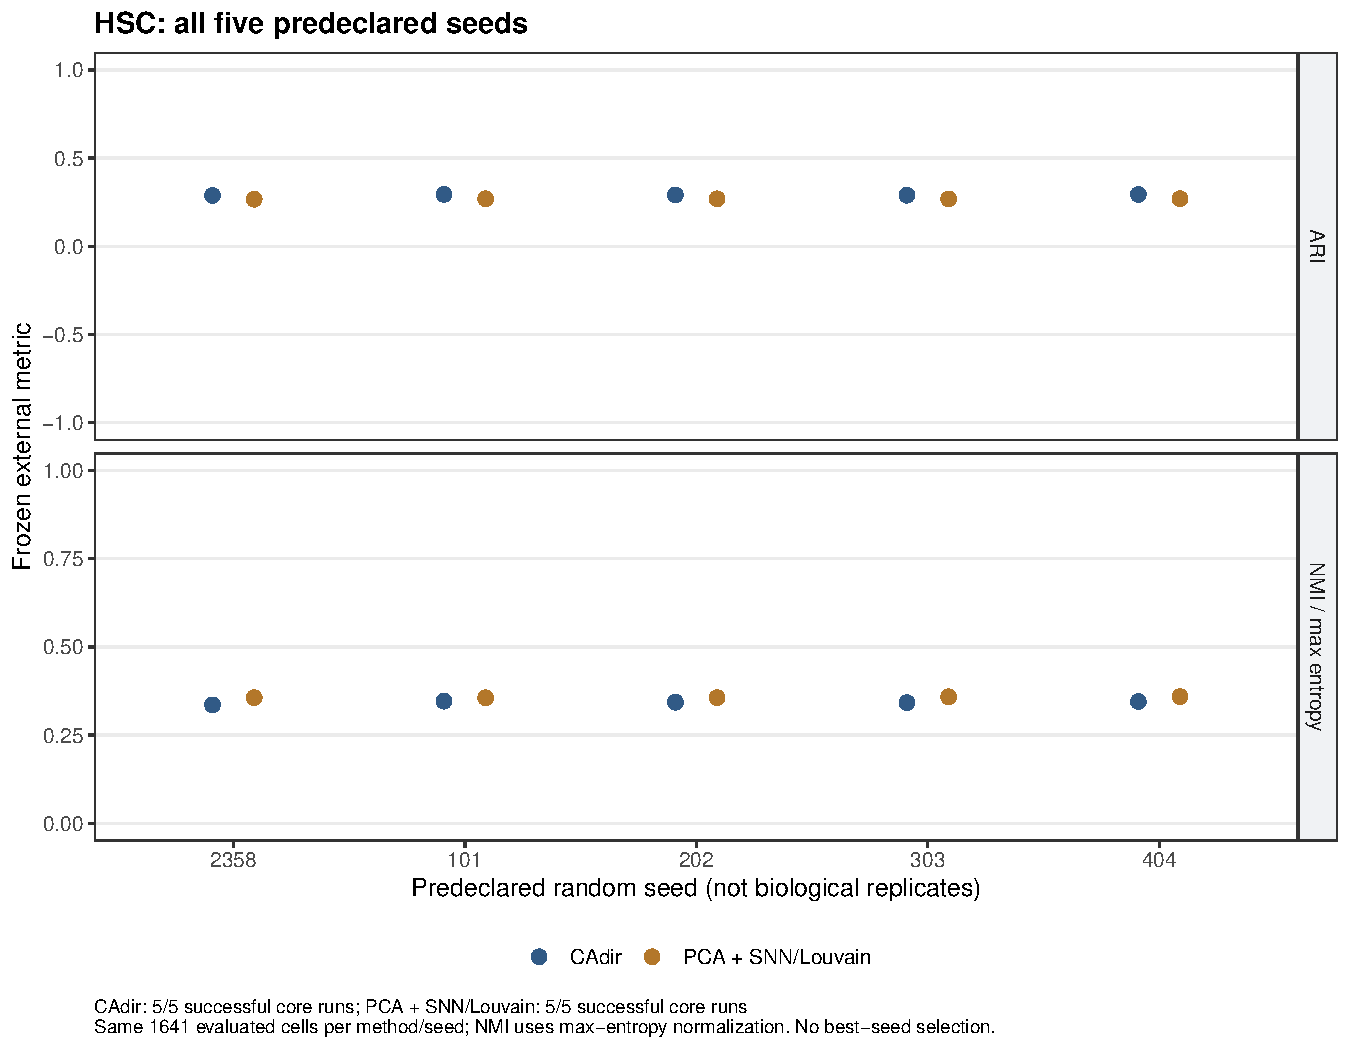
\includegraphics[width=0.96\textwidth,height=0.72\textheight,keepaspectratio]{figures/HSC_01-all-seed-ARI-NMI.pdf}
\caption{HSC两方法五种子ARI与NMImax}\label{fig:11}
\end{figure*}

\begin{table*}[!htbp]
\centering\zihao{-5}
\caption{HSC结果的中位数汇总}\label{tab:5}
\begin{tabularx}{\linewidth}{>{\raggedright\arraybackslash}X>{\raggedright\arraybackslash}X>{\raggedright\arraybackslash}X}
\toprule
指标 & CAdir & PCA＋SNN＋Louvain \\
\midrule
ARI & 0.291506398370853 & 0.269345381294258 \\
NMImax & 0.343414049181671 & 0.356463934525198 \\
核心耗时／秒 & 13.321 & 5.331 \\
最终簇数 & 9—11 & 7 \\
成功运行 & 5／5 & 5／5 \\
\bottomrule
\end{tabularx}
\end{table*}

核心耗时分别记录CA＋方向聚类和PCA＋rank-SNN＋Louvain，输出序列化与额外基因排名在各自记录中单独计时。

\subsection{结果解释}
CAdir的ARI中位数比基线高\allowbreak{}0.022161，NMImax中位数低\allowbreak{}0.013050。ARI从细胞对是否共同分组衡量一致性，并校正随机期望；NMImax以共享信息相对于较大分区熵归一化。CAdir产生\allowbreak{}9—11簇，基线产生\allowbreak{}7簇，聚类粒度与参考类别分布共同影响这两种度量，因而呈现不同排序。

以预定种子\allowbreak{}2358为展示例，图~\ref{fig:12}、13分别给出两种方法各簇的参考类别组成。它们配合完整列联表说明，整体指标背后同时存在单一类别占比较高的簇及包含多个参考类别的簇。五个种子提供计算初始化变化下的描述，所有种子均进入汇总。

\begin{figure*}[!tbp]
\centering
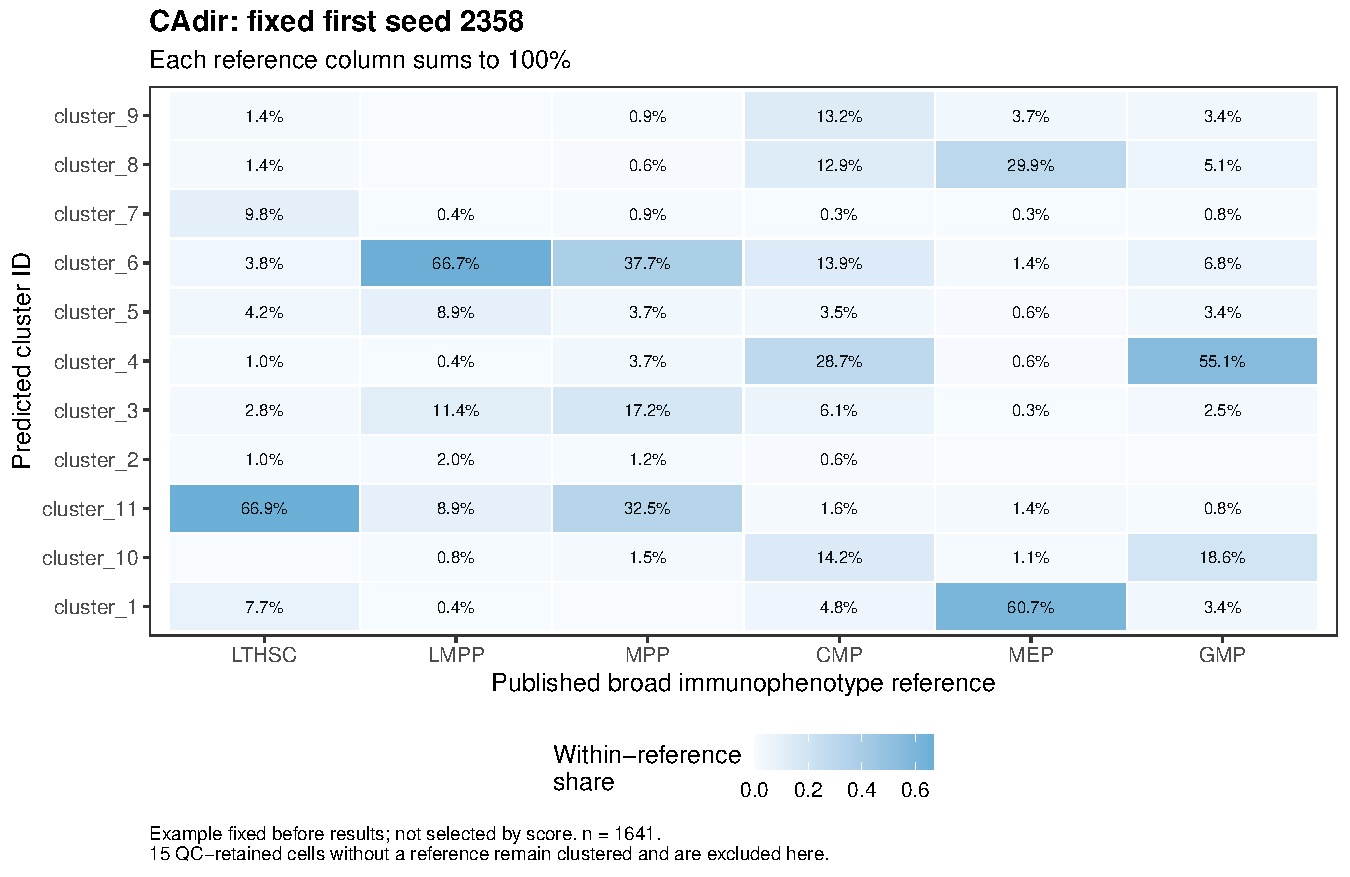
\includegraphics[width=0.96\textwidth,height=0.72\textheight,keepaspectratio]{figures/HSC_02-cadir-seed2358-reference-share.pdf}
\caption{HSC CAdir种子2358的簇内参考组成}\label{fig:12}
\end{figure*}

\begin{figure*}[!tbp]
\centering
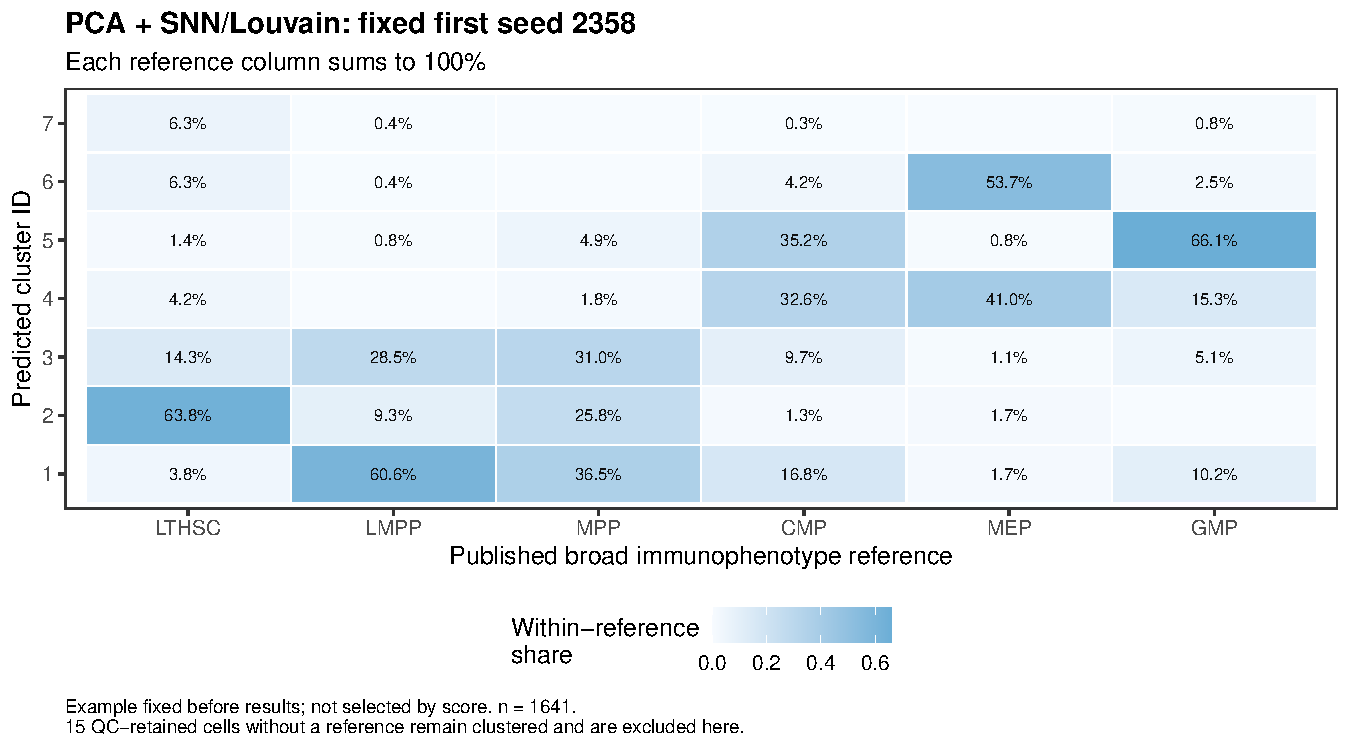
\includegraphics[width=0.96\textwidth,height=0.72\textheight,keepaspectratio]{figures/HSC_02-pca_snn_louvain-seed2358-reference-share.pdf}
\caption{HSC基线种子2358的簇内参考组成}\label{fig:13}
\end{figure*}

HSC结果的独立检查重新计算了十次指标，并检查保存对象、输入ID、输出完整性及主要图表。最大数值差异处于浮点舍入量级。

\section{综合讨论与实验体会}
\subsection{原论文案例与新数据之间的联系}
LM以组织类型相对明确的参考标签展示CAdir的联合输出：细胞簇、关联基因、自动名称及方向关系。HSC以造血干／祖细胞免疫表型标签开展方法比较，呈现出更细的预测分区和较低的参考一致性指标。两组实验分别回答“原案例怎样实现并解释”和“共享新输入下方法表现怎样”的问题。

LM的ARI为\allowbreak{}0.669519、HSC的CAdir中位ARI为\allowbreak{}0.291506。这些数值对应各自数据、标签和实际运行环境。LM的参考包含肌肉、间充质及免疫细胞，HSC的参考围绕造血干／祖细胞分化。比较结果时，应结合各自标签粒度、分区规模及几何展示解释。HSC同队列两方法对照提供了评价算法相对表现的直接依据。

\subsection{联合聚类的解释价值}
CAdir的价值体现在输出之间的连接。一个细胞方向对应一个分组，该分组关联一组基因，基因可按$S_\alpha$排序并参与富集，关联图显示聚类与基因的几何关系。LM的九图从单簇、簇间、历史和参考对应四个角度解释同一批对象，使读者可以逐层追踪结论。

图中名称按其生成方式解读：CellMarker提供GOA自动预测，原参考提供标签对应。内皮方向展示了自动注释在原参考粗类别内部给出的细分；B簇的混合参考组成展示了基因预测名与细胞标签之间的实际关系。保留这些结果有助于理解方法在不同信息来源下的表现。

\subsection{指标与可视化的互补}
ARI和NMI给出总体一致性，而关联图、方向角、流量和列联表定位具体差异。HSC中指标的不同排序说明，同时呈现两项评价能够提供更完整的描述。LM中巨噬细胞簇参考重叠较高，而B预测簇含有较多lymphocyte参考，进一步说明总体分数由不同局部结构共同构成。

\subsection{可重复计算与调试经验}
本次实验将输入文件哈希、明确ID、有效配置、实际CA对象、RNG、alpha与完整排名共同保存。基底符号问题的排查通过实际CA轴及排名变化得到解释，形成了固定／对齐基底下的排名重放方法。图表从保存对象生成，使数值计算、图形展示和版式修复各有明确输入。

实践中，脚本入口的Python层管理文件和状态，R层负责科学计算，JSON及TSV连接配置、指标和图表。按层保存对象及日志，使环境调试、数值检查和结果解释能够对应到具体阶段。独立数值复核则为图形和汇总指标提供了计算证据。

\section{结论}
本文完成了CAdir的LM原论文案例分析和HSC新数据对照实验。LM使用\allowbreak{}1882个细胞和\allowbreak{}6000个高变基因，得到\allowbreak{}7个细胞簇、1200个已分配基因，ARI为\allowbreak{}0.669519、NMImax为\allowbreak{}0.741885，完成原论文Fig3及关联S1的九项分析，核心汇总与作者公开运行记录对应。HSC采用共同QC、归一化、特征与评价集合，完成两方法各五种子实验，CAdir表现为ARI较高、NMImax较低及较细的预测分区。

方法分析与代码分析说明，CA提供细胞与基因的关联表示，方向分配与总最小二乘更新产生细胞分组，拆分合并调整簇数，基因排名与GOA连接分组和解释。实际对象、完整表格、九图、对照结果与独立检查记录共同构成了本报告的实验依据。
\par
